% !TEX root = ../thesis-main.tex
\part{\titleof{p3}}
\label{part3}
Generalization is at the heart of many aspects of human cognition. It underlies our ability to learn language, form and use categories, and learn about causal relationships, while in many cases we are presented only with limited observation. The great ability of generalization in human cognition sets a standard to which artificial intelligence and machine learning research aspires.

This immediately raises questions like ``How can human learn so much about the world from such limited evidence?'' and ``What makes human so good at generalization?''.
The importance of generalization in cognitive science partly derives
from its close relationship to inductive inference.  We can define generalization as forming predictions about future events based on examples from the past, which emphasizes its relationship to the classic problem of induction~\citep{hume2003treatise}. 
Having this connection between generalization and induction in mind, we can cast the question of ``how to produce good generalizations?'' to the question of ``what makes a good inductive learner?''.

To answer this question, from human cognition perspective, as human develop, they become capable of exploring ``more sophisticated hypotheses'' about the structure of their environment~\citep{inhelder1958growth}, which allows them to better infer their reality status and become better inductive learners. However, human sometimes has to make decisions without information from their senses or testimony from others, no matter how rich is their hypotheses space.
In these cases, their internal dispositions, i.e. ``inductive biases'', provides a source of knowledge that influences their decisions in the absence of experience, explicit sensory or testimonial proof~\cite{sodian1987children,griffiths2010probabilistic}.

In the context of learning algorithms, given the data $d$, the learner aims at identifying the hypothesis $h$ from a set of hypotheses $H$ that results in the highest generalization accuracy.  Having similar trend to the human cognition, algorithms that are able to explore ``richer hypothesis spaces'' have the potential of being better inductive learners\footnote{The idea of expansion of the hypothesis space by adding more layers and non-linearity to neural networks to make it possible to overcome the constraint of linear separability.}. However, in many cases, the considered hypotheses are not directly defined by the observed data and to choose among the many hypotheses that are equally granted by the data, the learner has to inject some preferences for those hypotheses that are called ``inductive biases''~\footnote{Biases can be both in inductive and in deductive systems. Systems that learn concepts from labeled training instances employ \emph{inductive bias}}. 

\emph{Inductive biases} are, in fact, factors that lead a learner to favor one hypothesis over another that are independent of the observed data. When two hypotheses fit the data equally well, inductive biases are the only basis for deciding between them and making it possible to generalize beyond the observed data~\citep{Mitchell80theneed}.

This brings us to the discussion of the \emph{bias-variance trade-off}.
We can decompose the expected generalization error into two parts: the
bias of a learning algorithm, and its variance~\citep{geman1992neural}. The transition from one source of error to another is known as the \emph{bias-variance trade-off}, and much of the research in designing learning algorithms is about trying to find the sweet spot between bias and variance for a given problem. 
%The generalization error can be attributed to a combination of intrinsic error due to the noise in output space, and systematic error resulting from the difference between the true function and the function selected by the learning algorithm.

The bias-variance trade-off suggests that the generalization of a learning algorithm depends on the problems at hand and different factors involved in learning, like the amount of available data. 
If the learner is provided with only small amounts of data, then the variance is the real concern and richer hypothesis spaces may hurt the generalization because they increase variance.  To increase the chance of generalization in these cases is to inject inductive biases with respect to the problem at hand.
However, if the learner is provided with large amounts of data and needs to be able to solve a variety of problems, then variance is less of an issue and the bias can be the dominant source of error, thus the learner needs richer hypothesis spaces to be flexible enough to accommodate the different solutions, as this reduces bias.

For neural networks, the inductive biases inherent in their architecture is perhaps the most important factor determining how quickly they train and how well they generalize beyond the data they observed during training. 
A well-known example is the translation invariant assumption in the convolutional neural networks~\citep{lecun1989backpropagation} for vision tasks based on a certain symmetry in the data, which considers that a given feature, of any complexity, can appear anywhere in the image.   Other examples include neural networks that encode rotational invariance~\citep{cohen2016steerable} or permutation invariance \citep{zaheer2017deep, lee2018set}.
Having inductive biases gets even more crucial when we need data \emph{efficient models} that are able to \emph{generalize beyond observed training data} and can \emph{learn complex tasks} like tasks that need reasoning or inferring an underlying structure from the data.

Among the sequence processing neural networks, recurrent neural networks have long been the de facto choice for sequence modeling tasks. The most important facet of RNNs is the \emph{recurrence} which lets the model updates its internal state in a loop given the input at each time step. The recurrence is simply using information from the previous state which in turn uses the previous state so on and so forth.  In other words, RNNs implement the ``re-occurrence'' of referring back to all previous internal states. This adds a ``recurrent inductive bias'' to the model that may be crucial for several algorithmic and language understanding tasks~\cite{tran2016recurrent,Dehghani:ICLR:2019}.

However, the recurrence in time dictates the inherently sequential computation which makes RNNs slow to train. Feed-forward and convolutional architectures have recently been shown to achieve superior results on some sequence modeling tasks such as machine translation~\citep{vaswani2017attention, NalBytenet2017}, with the added advantage that they concurrently process all inputs in the sequence, leading to easy parallelization and faster training times. Despite these successes, however, popular feed-forward sequence models like the Transformer~\citep{vaswani2017attention} fail to generalize in many simple tasks e.g. copying strings or even simple logical inference when the string or formula lengths exceed those observed at training time, while recurrent models handle these tasks with ease because of the inductive recurrent bias.

In Part~\ref{part3} of this thesis, we address the following research question:
\resq{p3}

Here, as a model with no recurrence in time, we focus on Transformer~\citep{vaswani2017attention} as a successful sequence model on many language understanding and generation tasks. In Chapter~\ref{chap:6}, we study how lack of recurrent inductive bias in Transformer may lead to the failure of the model on complex reasoning tasks with limited data, algorithmic tasks where length generalization over training samples is needed, and structured language understanding tasks, and address the following research question:
\resq{c6}

We introduced Universal Transformer~\citep{Dehghani:ICLR:2019}, a self-attentive concurrent-recurrent sequence model, which is an extension of Transformer model~\citep{vaswani2017attention}. The Universal Transformer introduces recurrence in depth by repeatedly refines a series of vector representations for each position of the sequence in parallel, by combining information from different positions using self-attention and applying a recurrent transition function across all time steps. 
In the simplest form, Universal Transformer with a fixed number of iterations is almost equivalent to a multi-layer Transformer with tied parameters across all its layers. By sharing weight, we can save massively on the number of parameters that we are training and fewer parameters means learn faster with fewer data points. We show that the elegant idea of introducing recurrent in depth enables Transformer to extrapolate from training data much better on a range of algorithmic and language understanding tasks~\cite{Dehghani:ICLR:2019, Dehghani:2019:WSDM}.

Besides the recurrence in depth, we propose a simple inductive bias for UTs that lets the model generalize well to input lengths that are not observed during training.  We also add a dynamic per-position halting mechanism and find that it improves accuracy on several tasks.  It is noteworthy that in contrast to the standard Transformer, under certain assumptions UTs can be shown to be \emph{Turing-complete}. We will discuss this further in Chapter~\ref{chap:6}.

% How can inductive biases be so strong yet so flexible? Nonparametric models, growing in complexity as the data require. 
\chapter{\titleof{c6}}
\blankfootnote{This chapter is based on \citep{Dehghani:ICLR:2019,Dehghani:2019:WSDM}.}

\label{chap:6}
%
\begin{quote}
Inductive biases are great ways for encoding modeling assumptions and improving data efficiency. For many sequence modeling tasks, the recurrent inductive bias plays a crucial role for generalizing beyond the observed data, while self-attentive feed-forward sequence models forego the recurrence toward parallelizability. We can, however, introduce a form of recurrent inductive bias to these models to improve their generalization while keeping the parallelization in the computations. 
\end{quote}
%

\section{Introduction}
Human child achieves the needed complex linguistic knowledge within a short time, with very limited observation. This cannot be explained easily and relying on the \emph{poverty of stimulus}~\citep{chomsky1980rules} argument, a powerful task-specific bias is required for learning to understand and generate language. In the context of learning algorithms, it has been discussed that without a certain complexity to the learning bias, the training data is insufficient to permit learning a model that generalizes properly to the full range of unseen instances for a specif task~\cite{Mitchell80theneed}. In other words, \emph{data-driven} learning, which merely relies on previous experience has to  with \emph{innately primed} learning, which is based on having the some knowledge encoded into the model in the form of fixed biases, either strong or weak.

Different neural network based models have been proposed for sequence modeling and and employed for language understanding and generation tasks. Among them, convolutional and fully-intentional feed-forward architectures like the Transformer have recently emerged as viable alternatives to recurrent neural networks (RNNs) for a range of sequence modeling tasks, notably machine translation~\citep{JonasFaceNet2017,transformer}. These parallel-in-time architectures address a significant shortcoming of RNNs, namely their inherently sequential computation which prevents parallelization across elements of the input sequence, whilst still addressing the vanishing gradients problem as the sequence length gets longer~\citep{vanishing-exploding-gradient}.
The Transformer model in particular relies entirely on a self-attention mechanism \citep{decomposableAttnModel,lin2017structured} to compute a series of context-informed vector-space representations of the symbols in its input and output, which are then used to predict distributions over subsequent symbols as the model predicts the output sequence symbol-by-symbol. Not only is this mechanism straightforward to parallelize, but as each symbol's representation is also directly informed by all other symbols' representations, this results in an effectively global receptive field across the whole sequence. This stands in contrast to e.g.,  convolutional architectures which typically only have a limited receptive field.

Notably, however, the Transformer with its fixed stack of distinct layers foregoes RNNs' inductive bias towards learning iterative or recursive transformations. Our experiments indicate that this inductive bias may be crucial for several algorithmic and language understanding tasks of varying complexity: in contrast to models such as the Neural Turing Machine~\citep{ntm14}, the Neural GPU~\citep{neural_gpu} or Stack RNNs~\citep{stack_rnn}, the Transformer does not generalize well to input lengths not encountered during training. 

In this chapter, we address the following research question:
\resq{c6}

\begin{figure}
 \centering
 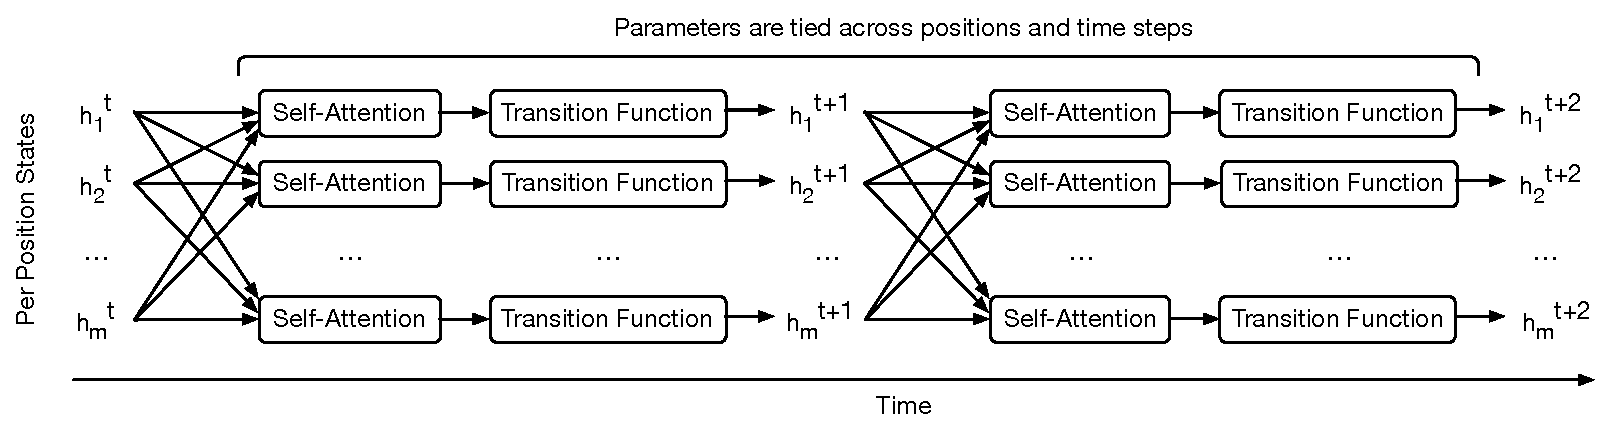
\includegraphics[width=\textwidth]{04-part-03/chapter-06/figs_and_tables/fig_universal-transformer-as-rnn.pdf}
 \caption{The Universal Transformer repeatedly refines a series of vector representations for each position of the sequence in parallel, by combining information from different positions using self-attention (see Eqn~\ref{MultiheadSelfAttention}) and applying a recurrent transition function (see Eqn~\ref{RecurrentTransition}) across all time steps $1 \leq t \leq T$. We show this process over two recurrent time-steps. Arrows denote dependencies between operations. Initially, $h^0$ is initialized with the embedding for each symbol in the sequence. $h^t_i$ represents the representation for input symbol $1 \leq i \leq m$ at recurrent time-step $t$. With dynamic halting, $T$ is dynamically determined for each position (Section~\ref{sec:dynamic-halting}).}
 \label{fig:rec-state}
\end{figure}


We introduce the \emph{Universal Transformer (UT)}, a parallel-in-time recurrent self-attentive sequence model which can be cast as a generalization of the Transformer model, yielding increased theoretical capabilities and improved results on a wide range of challenging sequence-to-sequence tasks. UTs combine the parallelizability and global receptive field of feed-forward sequence models like the Transformer with the recurrent inductive bias of RNNs, which seems to be better suited to a range of algorithmic and natural language understanding sequence-to-sequence problems. As the name implies, and in contrast to the standard Transformer, under certain assumptions UTs can be shown to be Turing-complete (or ``computationally universal'', as shown in Section~\ref{sec:related}).

In each recurrent step, the Universal Transformer iteratively refines its representations for all symbols in the sequence in parallel using a self-attention mechanism~\citep{decomposableAttnModel,lin2017structured}, followed by a transformation (shared across all positions and time-steps) consisting of a depth-wise separable convolution \citep{xception2016,slicenet} or a position-wise fully-connected layer (see Fig~\ref{fig:rec-state}). We also add a dynamic per-position halting mechanism \citep{graves2016adaptive}, allowing the model to choose the required number of refinement steps \emph{for each symbol} dynamically, and show for the first time that such a conditional computation mechanism can in fact improve accuracy on several smaller, structured algorithmic and linguistic inference tasks (although it marginally degraded results on MT). 

Our strong experimental results show that UTs outperform Transformers and LSTMs across a wide range of tasks. The added recurrence yields improved results in machine translation where UTs outperform the standard Transformer. In experiments on several algorithmic tasks and the bAbI language understanding task, UTs also consistently and significantly improve over LSTMs and the standard Transformer. Furthermore, on the challenging LAMBADA text understanding data set UTs with dynamic halting achieve a new state of the art.

\subsection{Detailed Research Questions}
We break down our main research question in this chapter into two concrete research questions:
\begin{resqbox}
\begin{enumerate}
\item[\textbf{\resqname{c6.1}}] \emph{\resqcontent{c6.1}}
\item[\textbf{\resqname{c6.2}}] \emph{\resqcontent{c6.2}}
\end{enumerate}
\end{resqbox}

In the following sections, we will address these research questions.

\section{The Universal Transformer }%: A Self-attentive Concurrent-Recurrent Sequence Model}
Here, in this section, we focus on the following research question:
\resq{c6.1}

The Universal Transformer (UT; see Fig.~\ref{fig:universal-transformer-complete}) is based on the popular encoder-decoder architecture commonly used in most neural sequence-to-sequence models \citep{sutskever14,cho2014learning,transformer}. Both the encoder and decoder of the UT operate by applying a recurrent neural network to the representations of each of the positions of the input and output sequence, respectively. However, in contrast to most applications of recurrent neural networks to sequential data, the UT does not recur over positions in the sequence, but over consecutive revisions of the vector representations of each position (i.e., over ``depth''). In other words, the UT is not computationally bound by the number of symbols in the sequence, but only by the number of revisions made to each symbol's representation.

In each recurrent time-step, the representation of every position is concurrently (in parallel) revised in two sub-steps: first, using a self-attention mechanism to exchange information across all positions in the sequence, thereby generating a vector representation for each position that is informed by the representations of all other positions at the previous time-step. Then, by applying a transition function (shared across position and time) to the outputs of the self-attention mechanism, independently at each position. As the recurrent transition function can be applied any number of times, this implies that UTs can have variable depth (number of per-symbol processing steps). Crucially, this is in contrast to most popular neural sequence models, including the Transformer~\citep{transformer} or deep RNNs, which have constant depth as a result of applying a \emph{fixed stack} of layers. We now describe the encoder and decoder in more detail.

\begin{figure}[t]
 \centering
 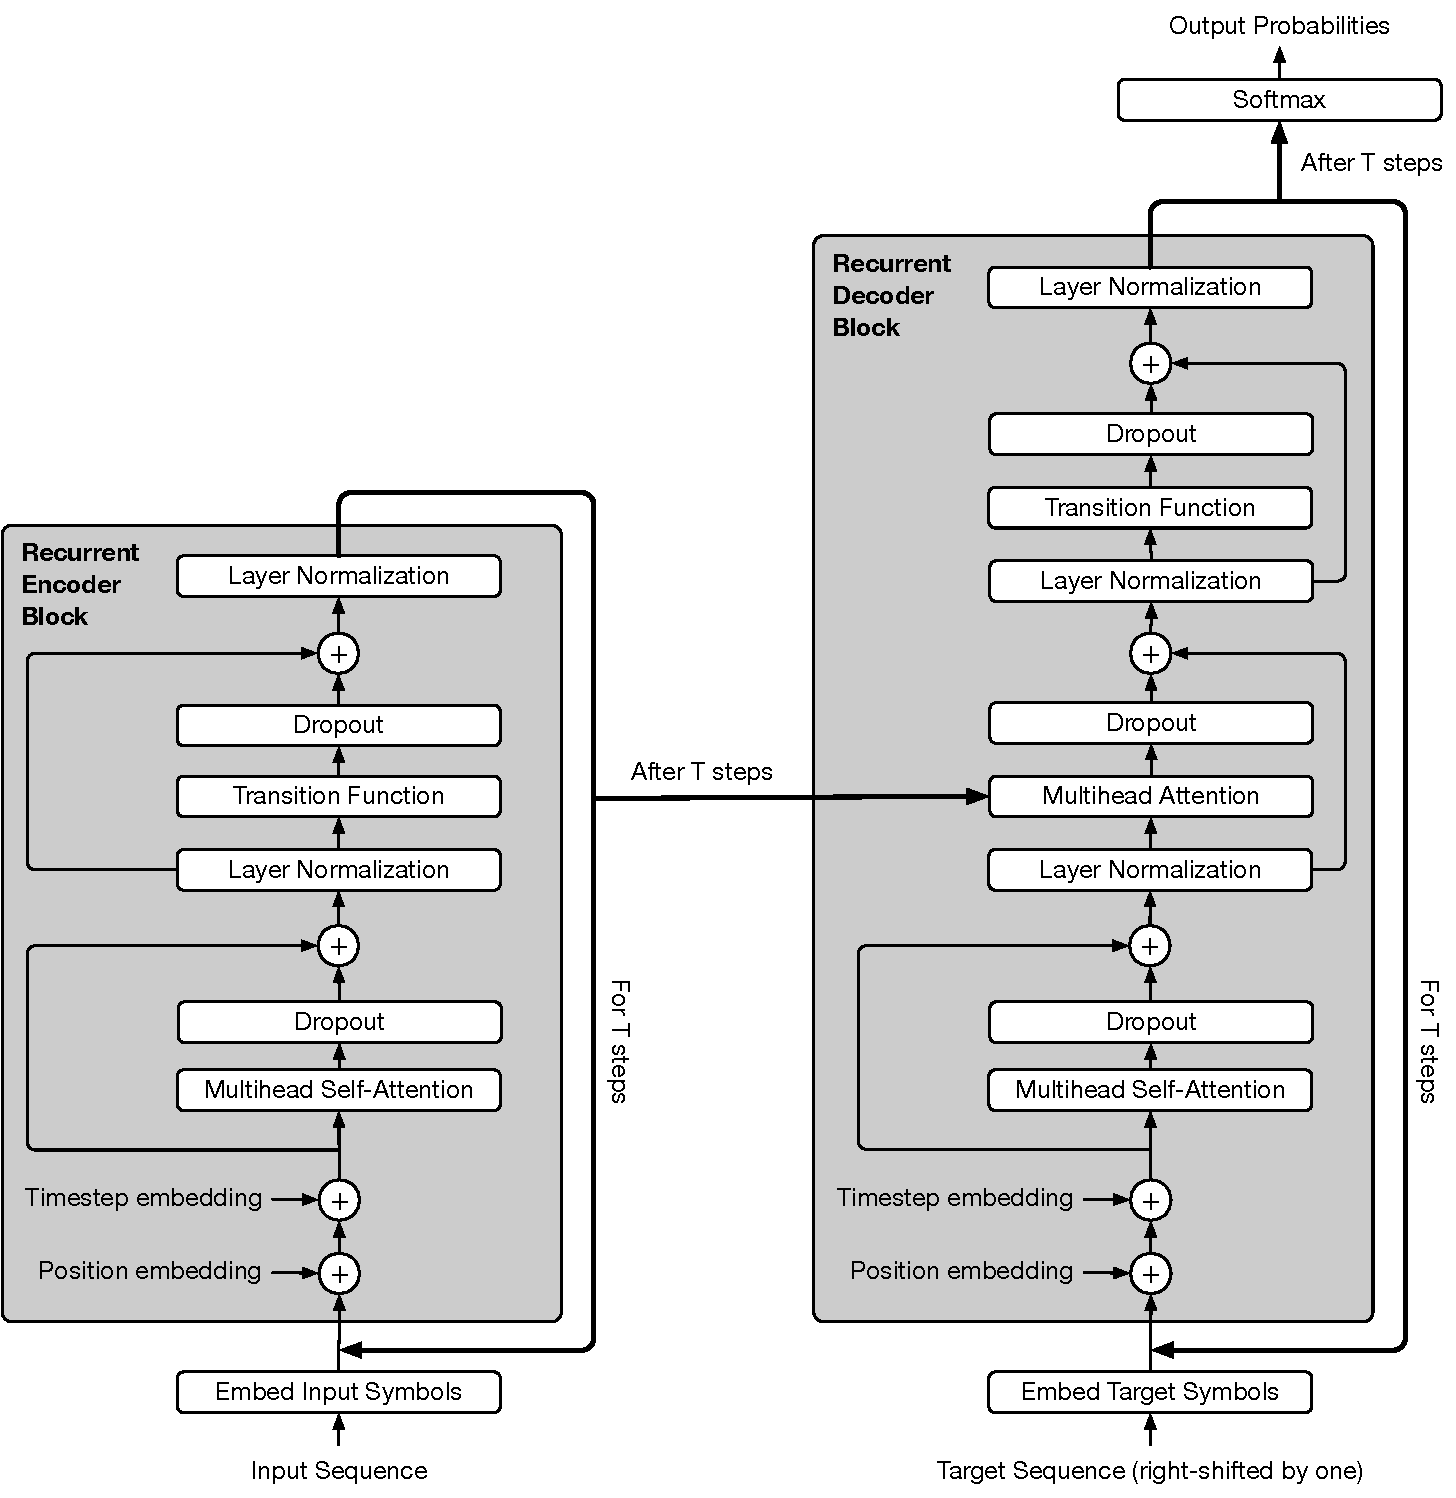
\includegraphics[width=0.9\textwidth]{04-part-03/chapter-06/figs_and_tables/fig_universal-transformer-complete.pdf}
 \caption{The recurrent blocks of the Universal Transformer encoder and decoder.}
 \label{fig:universal-transformer-complete}
\end{figure}

\textbf{\textsc{Encoder:}} Given an input sequence of length $m$, we start with a matrix whose rows are initialized as the $d$-dimensional embeddings of the symbols at each position of the sequence $H^0 \in \mathbb{R}^{m \times d}$. The UT then iteratively computes representations $H^t$ at step $t$ for all $m$ positions in parallel by applying the multi-headed dot-product self-attention mechanism from \cite{transformer}, followed by a recurrent transition function. We also add residual connections around each of these function blocks and apply dropout and layer normalization \citep{srivastava2014dropout, layernorm2016} (See Figure~\ref{fig:universal-transformer-complete} for the schema of the complete model.).

More specifically, we use the scaled dot-product attention which combines queries $Q$, keys $K$ and values $V$ as follows

\begin{equation}
   \textsc{Attention}(Q, K, V) = \textsc{softmax} \left( \frac{QK^T}{\sqrt{d}} \right) V,
\end{equation}

where $d$ is the number of columns of $Q$, $K$ and $V$. We use the multi-head version with $k$ heads, as introduced in \citep{transformer},

\begin{align}
    \label{MultiheadSelfAttention}
    \textsc{MultiHeadSelfAttention}(H^t) &= \textsc{Concat}(\mathrm{head_1}, ..., \mathrm{head_k})W^O\\
    \text{where}~\mathrm{head_i} &= \textsc{Attention}(H^t W^Q_i, H^t W^K_i, H^t W^V_i)
\end{align}

and we map the state $H^t$ to queries, keys and values with affine projections using learned parameter matrices $W^Q \in \mathbb{R}^{d \times d/k}$, $W^K \in \mathbb{R}^{d \times d/k}$, $W^V \in \mathbb{R}^{d \times d/k}$ and $W^O \in \mathbb{R}^{d \times d}$.

At step $t$, the UT then computes revised representations $H^t \in \mathbb{R}^{m \times d}$ for all $m$ input positions as follows

\begin{align}
    \label{RecurrentTransition}
    H^t &= \textsc{LayerNorm}(A^{t} + \textsc{Transition}(A^t) ) \\
    \mathrm{where}~A^t &= \textsc{LayerNorm}((H^{t-1} + P^{t}) + \textsc{MultiHeadSelfAttention}(H^{t-1} + P^{t})),
\end{align}
where \textsc{LayerNorm()} is defined in \cite{layernorm2016}, and \textsc{Transition()} and $P^t$ are discussed below.

Depending on the task, we use one of two different transition functions: either a separable convolution~\citep{xception2016} or a fully-connected neural network that consists of a single rectified-linear activation function between two affine transformations, applied position-wise, i.e., individually to each row of $A^t$.

$P^t \in \mathbb{R}^{m \times d}$ above are fixed, constant, two-dimensional (position, time) \emph{coordinate embeddings}, obtained by computing the sinusoidal position embedding vectors as defined in \citep{transformer} for the positions $1 \leq i \leq m$ and the time-step $1 \leq t \leq T$ separately for each vector-dimension $1 \leq j \leq d$, and summing:
\begin{align}
\label{eqn:coordinate-embeddings}
    P^t_{i, 2j} &= \sin(i / 10000^{2j / d}) + \sin(t / 10000^{2j / d}) \\
    P^t_{i, 2j+1} &= \cos(i / 10000^{2j / d}) + \cos(t / 10000^{2j / d}).
\end{align}

After $T$ steps (each updating all positions of the input sequence in parallel), the final output of the Universal Transformer encoder is a matrix of $d$-dimensional vector representations $H^T \in \mathbb{R}^{m \times d}$ for the $m$ symbols of the input sequence.

\textbf{\textsc{Decoder:}} The decoder shares the same basic recurrent structure of the encoder. However, after the self-attention function, the decoder additionally also attends to the final encoder representation $H^T$ of each position in the input sequence using the same multihead dot-product attention function from Equation \ref{MultiheadSelfAttention}, but with queries $Q$ obtained from projecting the decoder representations, and keys and values ($K$ and $V$) obtained from projecting the encoder representations (this process is akin to standard attention \citep{bahdanau2014neural}).

Like the Transformer model, the UT is autoregressive \citep{graves2013generating}. Trained using teacher-forcing, at generation time it produces its output one symbol at a time, with the decoder consuming the previously produced output positions. During training, the decoder input is the target output, shifted to the right by one position.
The decoder self-attention distributions are further masked so that the model can only attend to positions to the left of any predicted symbol. Finally, the per-symbol target distributions are obtained by applying an affine transformation $O \in \mathbb{R}^{d \times V}$ from the final decoder state to the output vocabulary size $V$, followed by a softmax which yields an $(m \times V)$-dimensional output matrix normalized over its rows:

\begin{equation}
 p\left(y_{pos} | y_{[1:pos - 1]}, H^T\right) = \textsc{softmax}(OH^T)\footnote{Note that $T$ here denotes time-step $T$ and not the transpose operation.}
\end{equation}

To generate from the model, the encoder is run once for the conditioning input sequence. Then the decoder is run repeatedly, consuming all already-generated symbols, while generating one additional distribution over the vocabulary for the symbol at the next output position per iteration. We then typically sample or select the highest probability symbol as the next symbol.


\subsection{Adaptive Computation by Dynamic Halting}
\label{sec:dynamic-halting}
\begin{figure}
 \centering
 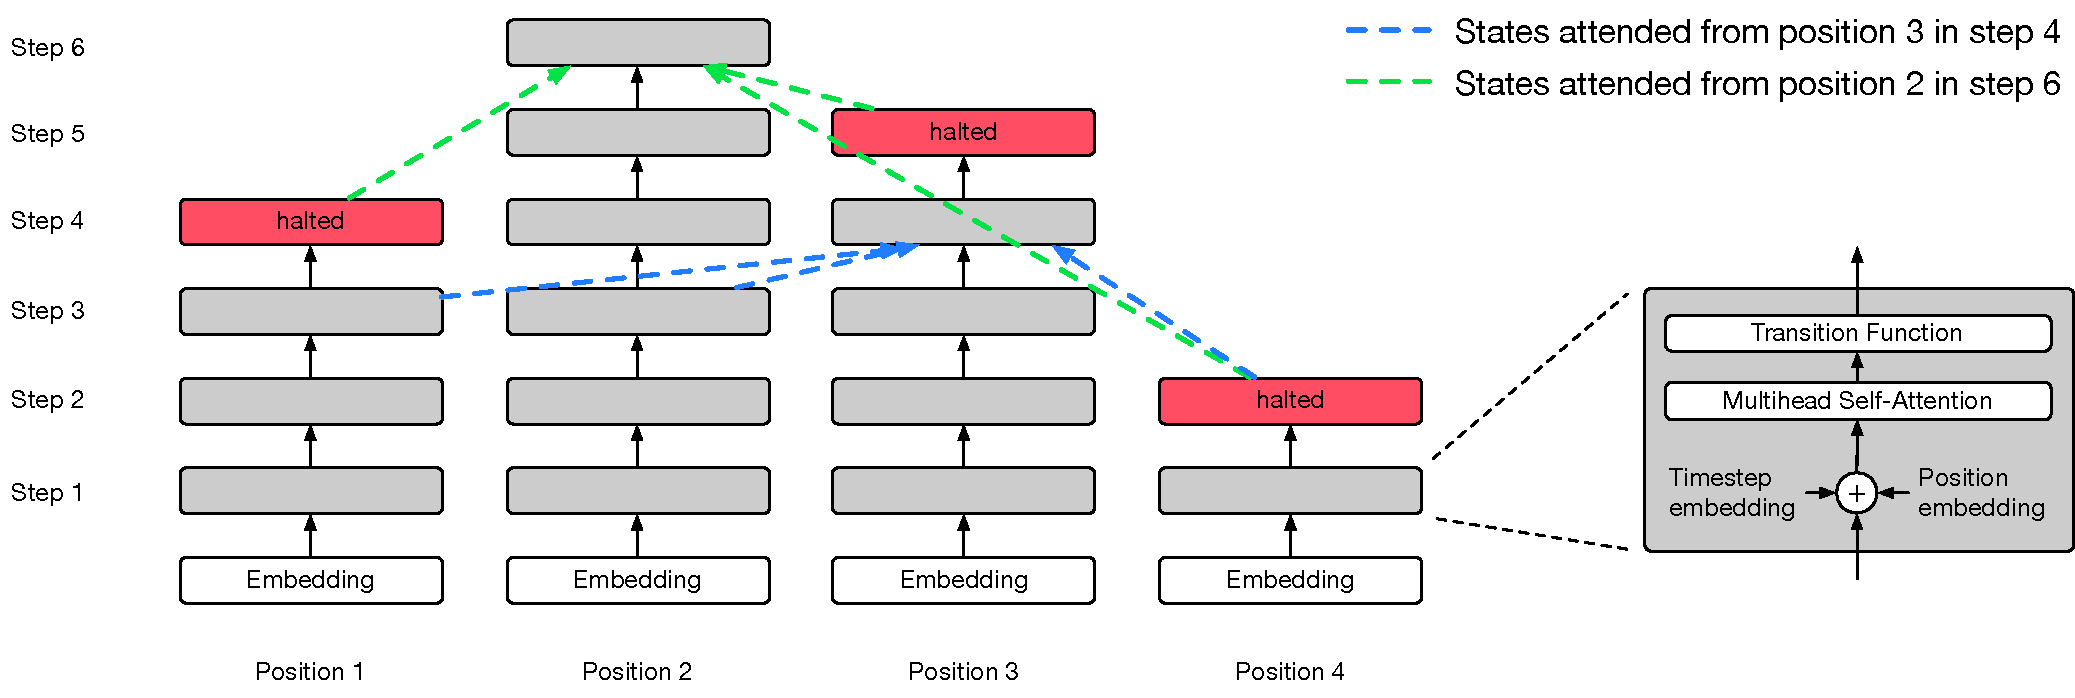
\includegraphics[width=1.0\textwidth]{04-part-03/chapter-06/figs_and_tables/fig_adaptive-universal-transformer.pdf}
 \caption{An unrolled visualization of Universal Transformer with dynamic halting. It illustrates different numbers of recurrent revisions per position (best viewed in colour).}
 \label{fig:adaptive_ut}
\end{figure}
In sequence processing systems, certain symbols (e.g., some words or phonemes) are usually more ambiguous than others. It is therefore reasonable to allocate more processing resources to these more ambiguous symbols. Adaptive Computation Time (ACT) \citep{graves2016adaptive} is a mechanism for dynamically modulating the number of computational steps needed to process each input symbol (called the ``ponder time'') in standard recurrent neural networks based on a scalar \emph{halting probability} predicted by the model at each step.

Inspired by the interpretation of Universal Transformers as applying self-attentive RNNs in parallel to all positions in the sequence, we also add a dynamic ACT halting mechanism to each position, i.e., to each per-symbol self-attentive RNN. Once the per-symbol recurrent block halts, its state is simply copied to the next step until all blocks halt, or we reach a maximum number of steps. The final output of the encoder is then the final layer of representations produced in this way. Figure~\ref{fig:adaptive_ut} illustrates a Universal Transformer encoder with $T$, number of revisions, dynamically determined for each position.


We implement the dynamic halting based on ACT~\citep{graves2016adaptive} as follows in TensorFlow. In each step of the UT with dynamic halting, we are given the halting probabilities, remainders, number of updates up to that point, and the previous state (all initialized as zeros), as well as a scalar threshold between 0 and 1 (a hyper-parameter). We then compute the new state for each position and calculate the new per-position halting probabilities based on the state for each position~\footnote{The current implementation of adaptive computation time does not allow for a fully ``end-to-end backpropable'' gradient of the proposed training loss. However, the discontinuity of the cost function might not imply that meaningful learning is not possible and in fact, the experiments in the original paper~\citep{graves2016adaptive} as well as here in Universal Transformer with adaptive halting suggest it works fine.}. The UT then decides to halt for some positions that crossed the threshold, and updates the state of other positions until the model halts for all positions or reaches a predefined maximum number of steps:
\begin{lstlisting}[language=Python, caption=UT with dynamic halting.]
# While-loop stops when this predicate is FALSE
# i.e. all ((probability < threshold) & (counter < max_steps)) are false
def should_continue(u0, u1, halting_probability, u2, n_updates, u3):
return tf.reduce_any(
            tf.logical_and(
                tf.less(halting_probability, threshold),
                tf.less(n_updates, max_steps)))
# Do while loop iterations until predicate above is false
(_, _, _, remainder, n_updates, new_state) = tf.while_loop(
    should_continue, ut_with_dynamic_halting, (state, 
    step, halting_probability, remainders, n_updates, previous_state))
\end{lstlisting}


% \begin{lstlisting}[language=Python, caption=]
%  # initializing halting probabilities
% halting_probability = tf.zeros(
%   (
%       batch_size,
%       length,
%   ), name="halting_probability")
% # initializing remainders 
% remainders = tf.zeros(
%   (
%       batch_size,
%       length,
%   ), name="remainder")
% # initializing number of updates performed 
% n_updates = tf.zeros(
%   (
%       batch_size,
%       length,
%   ), name="n_updates")

% # initializing Previous cell states
% previous_state = tf.zeros_like(state, name="previous_state")
% step = tf.constant(0, dtype=tf.int32)

% # While loop stops when this predicate is FALSE.
% # Ie all (probability < 1-eps AND counter < N) are false.
% def should_continue(u0, u1, halting_probability, u2, n_updates, u3):
% return tf.reduce_any(
%     tf.logical_and(
%         tf.less(halting_probability, threshold),
%         tf.less(n_updates, act_max_steps)))

% # Do while loop iterations until predicate above is false.
% (_, _, _, remainder, n_updates, new_state) = tf.while_loop(
%   should_continue, ut_with_dynamic_halting,
%   (state, step, halting_probability, remainders, n_updates, previous_state))
% \end{lstlisting}


The following shows the computations in each step:

\begin{lstlisting}[language=Python, caption=Computations in each step of the UT with dynamic halting.]
def ut_with_dynamic_halting(state, step, halting_probability, 
                            remainders, n_updates, previous_state):
    # Calculate the probabilities based on the state 
    p = common_layers.dense(state, 1, activation=tf.nn.sigmoid, 
        use_bias=True)
    # Mask for inputs which have not halted yet
    still_running = tf.cast(
        tf.less(halting_probability,1.0), tf.float32)
    # Mask of inputs which halted at this step
    new_halted = tf.cast(
        tf.greater(halting_probability + p * still_running, threshold), 
            tf.float32) * still_running
    # Mask of inputs which haven't halted, and didn't halt this step
    still_running = tf.cast(
        tf.less_equal(halting_probability + p * still_running, 
            threshold), tf.float32) * still_running
    # Add the halting probability for this step to the halting
    # probabilities for those inputs which haven't halted yet
    halting_probability += p * still_running
    # Compute remainders for the inputs which halted at this step
    remainders += new_halted * (1 - halting_probability)
    # Add the remainders to those inputs which halted at this step
    halting_probability += new_halted * remainders
    # Increment n_updates for all inputs which are still running
    n_updates += still_running + new_halted
    # Compute the weight to be applied to the new state and output:
    #   0 when the input has already halted,
    #   p when the input hasn't halted yet,
    #   the remainders when it halted this step.
    update_weights = tf.expand_dims(p * still_running +
                                    new_halted * remainders, -1)
    # Apply transformation to the state
    transformed_state = transition_function(self_attention(state))
    # Interpolate transformed and previous states for non-halted inputs
    new_state = ((transformed_state * update_weights) +
                 (previous_state * (1 - update_weights)))
    step += 1
    return (transformed_state, step, halting_probability,
            remainders, n_updates, new_state)
\end{lstlisting}


\section{Universality and Relation to other Models}
\label{sec:related}
When running for a fixed number of steps, the Universal Transformer is equivalent to a multi-layer Transformer with tied parameters across all its layers. This is partly similar to the Recursive Transformer, which ties the weights of its self-attention layers across depth~\citep{gulcehre2018hyperbolic}\footnote{Note that in UT both the self-attention and transition weights are tied across layers.}. However, as the per-symbol recurrent transition functions can be applied any number of times, another and possibly more informative way of characterizing the UT is as a block of parallel RNNs (one for each symbol, with shared parameters) evolving per-symbol hidden states concurrently, generated at each step by attending to the sequence of hidden states at the previous step. In this way, it is related to architectures such as the Neural GPU \citep{neural_gpu} and the Neural Turing Machine \citep{ntm14}. UTs thereby retain the attractive computational efficiency of the original feed-forward Transformer model, but with the added recurrent inductive bias of RNNs. Furthermore, using a dynamic halting mechanism, UTs can choose the number of processing steps based on the input data. %interpolate between the feed-forward, fixed-depth Transformer and a gated, recurrent architecture running for a number of steps dependent on the input data. 

The connection between the Universal Transformer and other sequence models is apparent from the architecture: if we limited the recurrent steps to one, it would be a Transformer. But it is more interesting to consider the relationship between the Universal Transformer and RNNs and other networks where recurrence happens over the time dimension. Superficially these models may seem closely related since they are recurrent as well. But there is a crucial difference: time-recurrent models like RNNs cannot access memory in the recurrent steps. This makes them computationally more similar to automata, since the only memory available in the recurrent part is a fixed-size state vector. UTs, on the other hand, can attend to the whole previous layer, allowing it to access memory in the recurrent step. 

Given sufficient memory the Universal Transformer is computationally universal -- i.e., it belongs to the class of models that can be used to simulate any Turing machine, thereby addressing a shortcoming of the standard Transformer model. In addition to being theoretically appealing, our results show that this added expressivity also leads to improved accuracy on several challenging sequence modeling tasks. This closes the gap between practical sequence models competitive on large-scale tasks such as machine translation, and computationally universal models such as the Neural Turing Machine or the Neural GPU \citep{ntm14,neural_gpu}, which can be trained using gradient descent to perform algorithmic tasks.

To show this, we can reduce a Neural GPU to a Universal Transformer. Ignoring the decoder and parameterizing the self-attention module, i.e., self-attention with the residual connection, to be the identity function, we assume the transition function to be a convolution. If we now set the total number of recurrent steps $T$ to be equal to the input length, we obtain exactly a Neural GPU. Note that the last step is where the Universal Transformer crucially differs from the vanilla Transformer whose depth cannot scale dynamically with the size of the input. A similar relationship exists between the Universal Transformer and the Neural Turing Machine, whose single read/write operations per step can be expressed by the global, parallel representation revisions of the Universal Transformer. In contrast to these models, however, which only perform well on algorithmic tasks, the Universal Transformer also achieves competitive results on realistic natural language tasks such as LAMBADA and machine translation.

Another related model architecture is that of end-to-end Memory Networks \citep{sukhbaatar2015}. In contrast to end-to-end memory networks, however, the Universal Transformer uses memory corresponding to states aligned to individual positions of its inputs or outputs. Furthermore, the Universal Transformer follows the encoder-decoder configuration and achieves competitive performance in large-scale sequence-to-sequence tasks.


\subsection{On the Computational Power of UT vs Transformer}
\label{app:univerrality_example}

With respect to their computational power, the key difference between the Transformer and the Universal Transformer lies in the number of sequential steps of computation (i.e., in depth). While a standard Transformer executes a total number of operations that scales with the input size, the number of sequential operations is constant, independent of the input size and determined solely by the number of layers. Assuming finite precision, this property implies that the standard Transformer cannot be computationally universal. When choosing a number of steps as a function of the input length, however, the Universal Transformer does not suffer from this limitation. Note that this holds independently of whether or not adaptive computation time is employed but does assume a non-constant, even if possibly deterministic, number of steps. Varying the number of steps dynamically after training is enabled by sharing weights across sequential computation steps in the Universal Transformer.

\begin{figure}[t]
\centering
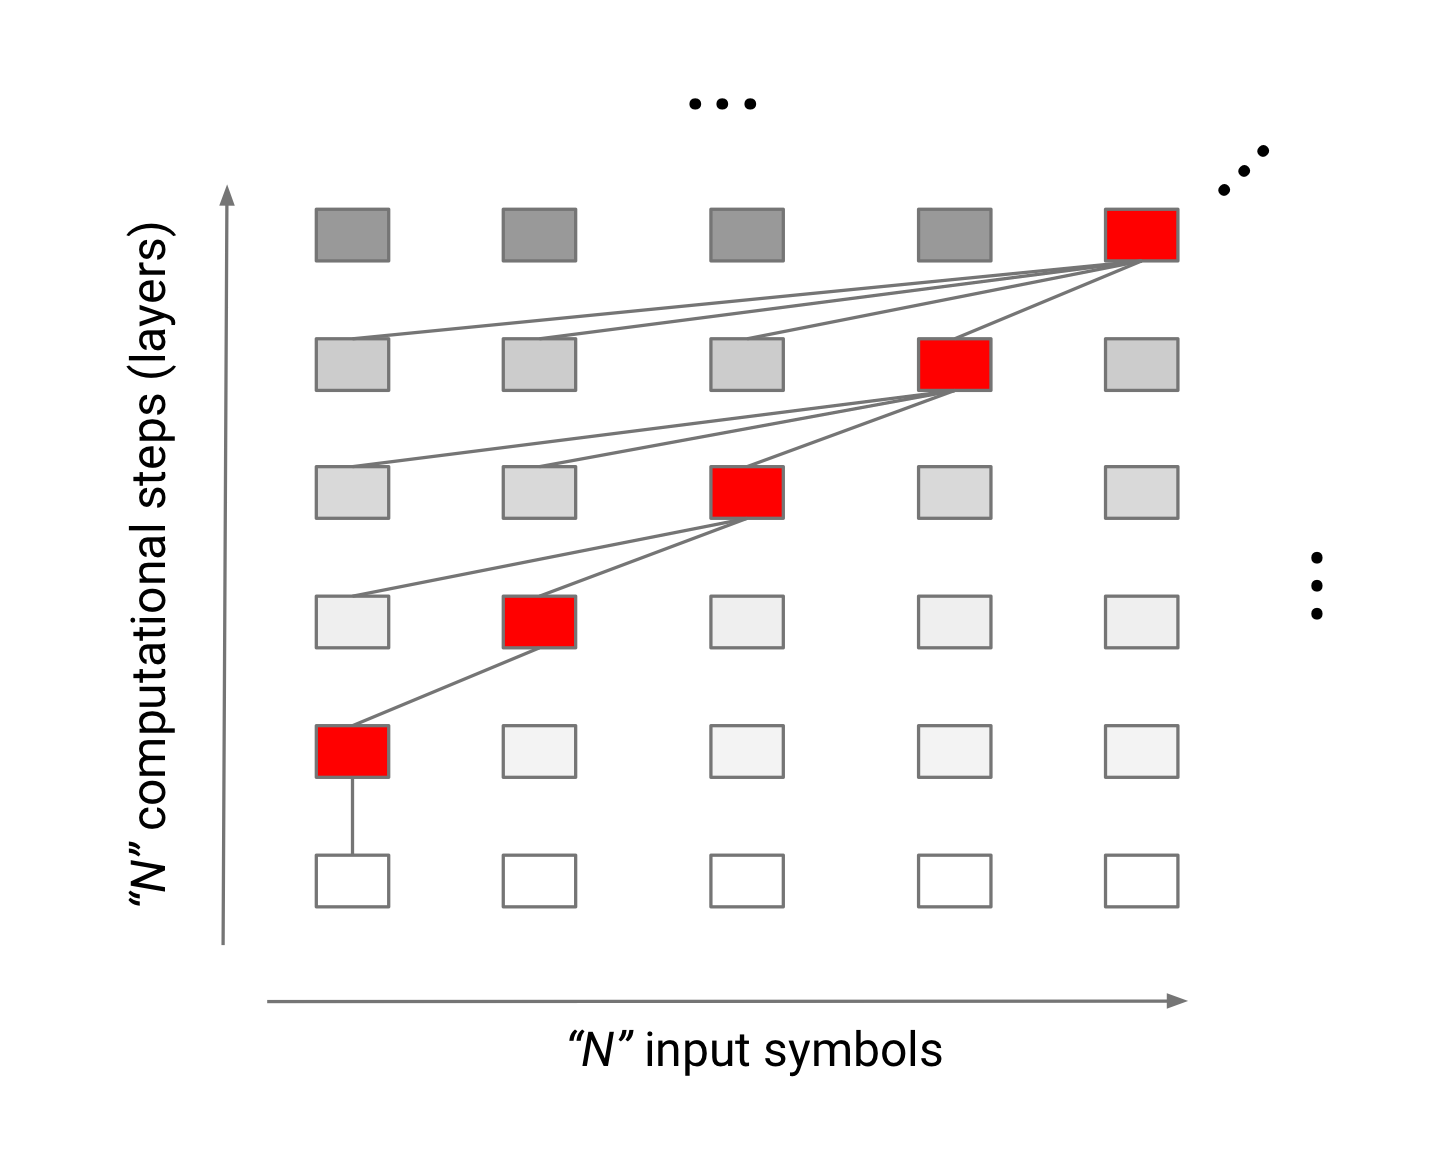
\includegraphics[width=0.6\textwidth, trim={0.1cm 0.5cm 0.1cm 1.2cm}, clip]{04-part-03/chapter-06/figs_and_tables/fig_universality_example.png}
\end{figure}

An intuitive example are functions whose execution requires the sequential processing of each input element. In this case, for any given choice of depth $T$, one can construct an input sequence of length $N>T$ that cannot be processed correctly by a standard Transformer. With an appropriate, input-length dependent choice of sequential steps, however, a Universal Transformer, RNNs or Neural GPUs can execute such a function.
\section{Universal Transformer for Sequence Modeling}
In this section, we address the following research question:
\resq{c6.2}
We evaluate Universal Transformers on a range of algorithmic and language understanding tasks and discuss the results. In the tasks that are chosen, we include some with limited number of training samples, or some with incomplete training set (lack of converge), but also tasks that do not suffer severely from imperfect supervision, to evaluate the performance of our model in both situations. 

\subsection{bAbI Question-Answering}
The bAbi question answering dataset~\citep{weston2015towards} consists of 20 different synthetic tasks\footnote{\url{https://research.fb.com/downloads/babi}}. The aim is that each task tests a unique aspect of language understanding and reasoning, including the ability of: reasoning from supporting facts in a story, answering true/false type questions, counting, understanding negation and indefinite knowledge, understanding coreferences, time reasoning, positional and size reasoning, path-finding, and understanding motivations (to see examples for each of these tasks, please refer to Table 1 in \citep{weston2015towards}).

There are two versions of the dataset, one with 1k training samples and the other with 10k samples. It is important for a model to be data-efficient to achieve good results using only the 1k training samples. Moreover, the original idea is that a single model should be evaluated across all the tasks (not tuning per task), which is the \emph{train joint} setup in Tables~\ref{tab:babi-results} and ~\ref{tbl:babi_details}.

Solving all the bAbI tasks by training a model on the 1k training dataset is pretty challenging as some of the tasks are rather complex and with only 1k samples for each task, its hard for most of models to generalize well. So data efficiency should be a key property to be considered here. 
We tried a standard Transformer and observed that it does not achieve good results on bAbI tasks\footnote{We experimented with different hyper-parameters and different network sizes, but it always overfits.}. However, we have designed a model based on the Universal Transformer which achieves state-of-the-art results bAbI task. 
This is mainly due to recurrent inductive bias in the Universal Transformer as well as the fact that sharing parameters across depth decreases the number of parameters which helps the model generalize better.

To encode the input, similar to~\cite{henaff2016tracking}, we first encode each fact in the story by applying a learned multiplicative positional mask to each word's embedding, and summing up all embeddings.
We embed the question in the same way, and then feed the (Universal) Transformer with these embeddings of the facts and questions. 

As originally proposed, models can either be trained on each task separately (``train single'') or jointly on all tasks (``train joint''). Table~\ref{tab:babi-results} summarizes our results. We conducted 10 runs with different initializations and picked the best model based on performance on the validation set, similar to previous work. Both the UT and UT with dynamic halting achieve state-of-the-art results on all tasks in terms of average error and number of failed tasks\footnote{Defined as $> 5\%$ error.}, in both the 10K and 1K training regime. Tables~\ref{tbl:babi_details} presents the results of best and average results of 10 runs breakdown by task.

\begin{table}[t!]
\centering
\begin{adjustbox}{max width=\textwidth}
\begin{tabular}{lllll}
& & & & \\ \toprule
\multirow{2}{*}{ \bf Model } & \multicolumn{2}{c}{ \bf 10K examples } & \multicolumn{2}{c}{ \bf 1K examples } \\ \cmidrule{2-5}
& train single & train joint & train single & train joint \\ \midrule
\multicolumn{5}{c}{\bf Previous best results:} \\ \midrule
QRNet~\citep{seo2016query} & 0.3 (0/20) & - & - & - \\
Sparse DNC~\citep{rae2016scaling} & - & 2.9 (1/20) & - & - \\
GA+MAGE~\cite{dhingra2017linguistic} & - & - & 8.7 (5/20) & - \\
MemN2N~\cite{sukhbaatar2015} & - & - & -  & 12.4 (11/20) \\\midrule
\multicolumn{5}{c}{\bf Our Results:} \\ \midrule
Transformer~\citep{transformer} & 15.2 (10/20) & 22.1 (12/20) & 21.8 (5/20) & 26.8 (14/20) \\
Universal Transformer (this work) & 0.23 (0/20) & 0.47 (0/20) & 5.31 (5/20) & 8.50 (8/20) \\
UT w/ dynamic halting (this work) & {\bf 0.21 (0/20)} & {\bf 0.29 (0/20)} & {\bf 4.55 (3/20)} & {\bf 7.78 (5/20)} \\ \bottomrule
\end{tabular}
\end{adjustbox}
\caption{Average error and number of failed tasks ($> 5\%$ error) out of 20 (in parentheses; lower is better in both cases) on the bAbI dataset under the different training/evaluation setups. We indicate state-of-the-art where available for each, or `-' otherwise.}
\label{tab:babi-results}
\end{table}
\begin{table}[t!]
\centering
\caption{Detailed results on the bAbI question answering tasks.}
\label{tbl:babi_details}
\begin{subtable}{0.6\textwidth}
\centering
\begin{adjustbox}{max width=\textwidth}
\begin{tabular}{lcccc}
\toprule
\multicolumn{5}{c}{Best seed run for each task (out of 10 runs) } \\ \midrule
\multirow{2}{*}{ Task id } & \multicolumn{2}{c}{ 10K } & \multicolumn{2}{c}{ 1K } \\  \cmidrule{2-5}
& train single & train joint & train single & train joint \\ \midrule
1 & 0.0 & 0.0 & 0.0 & 0.0 \\
2 & 0.0 & 0.0 & 0.0 & 0.5 \\
3 & 0.4 & 1.2 & 3.7 & 5.4 \\
4 & 0.0 & 0.0 & 0.0 & 0.0 \\
5 & 0.0 & 0.0 & 0.0 & 0.5 \\
6 & 0.0 & 0.0 & 0.0 & 0.5 \\
7 & 0.0 & 0.0 & 0.0 & 3.2 \\
8 & 0.0 & 0.0 & 0.0 & 1.6 \\
9 & 0.0 & 0.0 & 0.0 & 0.2 \\
10 & 0.0 & 0.0 & 0.0 & 0.4 \\
11 & 0.0 & 0.0 & 0.0 & 0.1 \\
12 & 0.0 & 0.0 & 0.0 & 0.0 \\
13 & 0.0 & 0.0 & 0.0 & 0.6 \\
14 & 0.0 & 0.0 & 0.0 & 3.8 \\
15 & 0.0 & 0.0 & 0.0 & 5.9 \\
16 & 0.4 & 1.2 & 5.8 & 15.4 \\
17 & 0.6 & 0.2 & 32.0 & 42.9 \\
18 & 0.0 & 0.0 & 0.0 & 4.1 \\
19 & 2.8 & 3.1 & 47.1 & 68.2 \\
20 & 0.0 & 0.0 & 2.4 & 2.4 \\ \midrule
avg err & 0.21 & 0.29 & 4.55 & 7.78 \\ \midrule
failed & 0 & 0 & 3 & 5 \\
\bottomrule
\end{tabular}
\end{adjustbox}
\end{subtable}
\\
\vspace{10pt}
\begin{subtable}{0.6\textwidth}
\centering
\begin{adjustbox}{max width=\textwidth}
\begin{tabular}{lcccc}
\toprule
\multicolumn{5}{c}{Average (\rpm var) over all seeds (for 10 runs)} \\ \midrule
\multirow{2}{*}{ Task id } & \multicolumn{2}{c}{ 10K } & \multicolumn{2}{c}{ 1K } \\  \cmidrule{2-5}
& train single & train joint & train single & train joint \\ \midrule
1 & 0.0 \rpm 0.0 & 0.0 \rpm 0.0 & 0.2 \rpm 0.3 & 0.1 \rpm 0.2 \\ 
2 & 0.2 \rpm 0.4 & 1.7 \rpm 2.6 & 3.2 \rpm 4.1 & 4.3 \rpm 11.6 \\ 
3 & 1.8 \rpm 1.8 & 4.6 \rpm 7.3 & 9.1 \rpm 12.7 & 14.3 \rpm 18.1 \\ 
4 & 0.1 \rpm 0.1 & 0.2 \rpm 0.1 & 0.3 \rpm 0.3 & 0.4 \rpm 0.6 \\ 
5 & 0.2 \rpm 0.3 & 0.8 \rpm 0.5 & 1.1 \rpm 1.3 & 4.3 \rpm 5.6 \\ 
6 & 0.1 \rpm 0.2 & 0.1 \rpm 0.2 & 1.2 \rpm 2.1 & 0.8 \rpm 0.4 \\ 
7 & 0.3 \rpm 0.5 & 1.1 \rpm 1.5 & 0.0 \rpm 0.0 & 4.1 \rpm 2.9 \\ 
8 & 0.3 \rpm 0.2 & 0.5 \rpm 1.1 & 0.1 \rpm 0.2 & 3.9 \rpm 4.2 \\ 
9 & 0.0 \rpm 0.0 & 0.0 \rpm 0.0 & 0.1 \rpm 0.1 & 0.3 \rpm 0.3 \\ 
10 & 0.1 \rpm 0.2 & 0.5 \rpm 0.4 & 0.7 \rpm 0.8 & 1.3 \rpm 1.6 \\ 
11 & 0.0 \rpm 0.0 & 0.1 \rpm 0.1 & 0.4 \rpm 0.8 & 0.3 \rpm 0.9 \\ 
12 & 0.2 \rpm 0.1 & 0.4 \rpm 0.4 & 0.6 \rpm 0.9 & 0.3 \rpm 0.4 \\ 
13 & 0.2 \rpm 0.5 & 0.3 \rpm 0.4 & 0.8 \rpm 0.9 & 1.1 \rpm 0.9 \\ 
14 & 1.8 \rpm 2.6 & 1.3 \rpm 1.6 & 0.1 \rpm 0.2 & 4.7 \rpm 5.2 \\ 
15 & 2.1 \rpm 3.4 & 1.6 \rpm 2.8 & 0.3 \rpm 0.5 & 10.3 \rpm 8.6 \\ 
16 & 1.9 \rpm 2.2 & 0.9 \rpm 1.3 & 9.1 \rpm 8.1 & 34.1 \rpm 22.8 \\ 
17 & 1.6 \rpm 0.8 & 1.4 \rpm 3.4 & 43.7 \rpm 18.6 & 51.1 \rpm 12.9 \\ 
18 & 0.3 \rpm 0.4 & 0.7 \rpm 1.4 & 2.3 \rpm 3.6 & 12.8 \rpm 9.0 \\ 
19 & 3.4 \rpm 4.0 & 6.1 \rpm 7.3 & 50.2 \rpm 8.4 & 73.1 \rpm 23.9 \\ 
20 & 0.0 \rpm 0.0 & 0.0 \rpm 0.0 & 3.2 \rpm 2.5 & 2.6 \rpm 2.8 \\ \midrule
avg & 0.73 \rpm 0.89 & 1.12 \rpm 1.62 & 6.34 \rpm 3.32 & 11.21 \rpm 6.65 \\ 
\bottomrule
\end{tabular}
\end{adjustbox}
\end{subtable}
\end{table}
\afterpage{\clearpage}


To understand the working of the model better, we analyzed both the attention distributions and the average ACT ponder times for this task. First, we observe that the attention distributions start out very uniform, but get progressively sharper in later steps around the correct supporting facts that are required to answer each question, which is indeed very similar to how humans would solve the task. 
%
Second, with dynamic halting we observe that the average ponder time (i.e., depth of the per-symbol recurrent processing chain) over all positions in all samples in the test data for tasks requiring three supporting facts is higher ($3.8 \rpm 2.2$) than for tasks requiring only two ($3.1 \rpm 1.1$), which is in turn higher than for tasks requiring only one supporting fact ($2.3 \rpm 0.8$). This indicates that the model adjusts the number of processing steps with the number of supporting facts required to answer the questions. 

\begin{figure}[t]
 \centering
 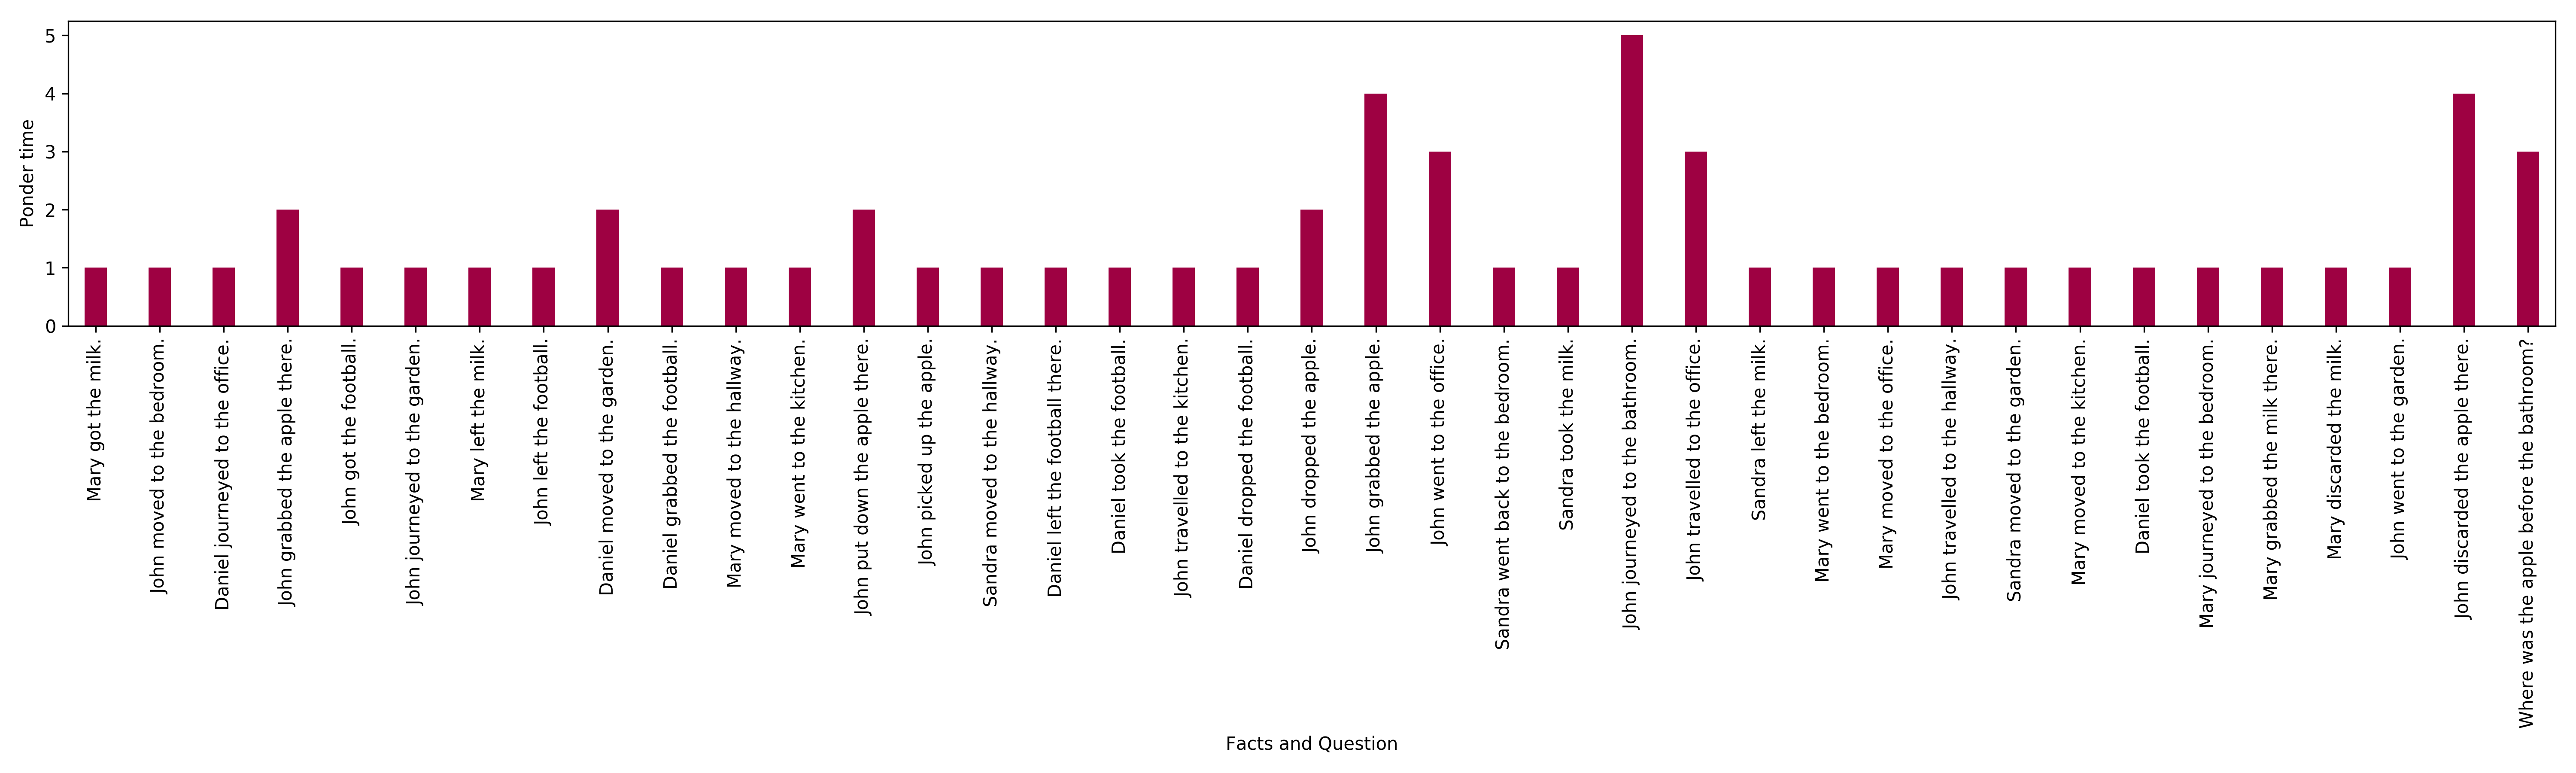
\includegraphics[width=\textwidth]{04-part-03/chapter-06/figs_and_tables/fig_task3_example_ponder.png}
 \caption{Ponder time of UT with dynamic halting for encoding facts in a story and question in a bAbI task requiring three supporting facts.}
 \label{fig:act_ponder}
\end{figure}
Finally, we observe that the histogram of ponder times at different positions is more uniform in tasks requiring only one supporting fact compared to two and three, and likewise for tasks requiring two compared to three.  Especially for tasks requiring three supporting facts, many positions halt at step 1 or 2 already and only a few get transformed for more steps (see, for example, Figure~\ref{fig:act_ponder}). This is particularly interesting as the length of stories is indeed much higher in this setting, with more irrelevant facts which the model seems to successfully learn to ignore in this way.

Similar to dynamic memory networks~\citep{kumar2016ask}, there is an iterative attention process in UTs that allows the model to condition its attention over memory on the result of previous iterations. 
%

\begin{figure}[!ht]
\begin{minipage}{\textwidth}
\fontsize{8}{8}\fontfamily{pcr}\selectfont
\begin{tabular}{l l}
\textbf{An example from tasks 1}: & \textbf{(requiring one supportive fact to solve)}\\
\\
\textbf{Story}: & \\
& John travelled to the hallway. \\
& Mary journeyed to the bathroom. \\
& Daniel went back to the bathroom. \\
& John moved to the bedroom \\
\\
\textbf{Question}: & \\
& Where is Mary? \\
\textbf{Model's output}: & \\
& bathroom
\end{tabular}
\end{minipage}
\\ \vfill
\vspace{20pt} % maximize space between the minipages
\begin{minipage}{\textwidth}
    \centering
    \begin{subfigure}[t]{\textwidth}
        \centering
        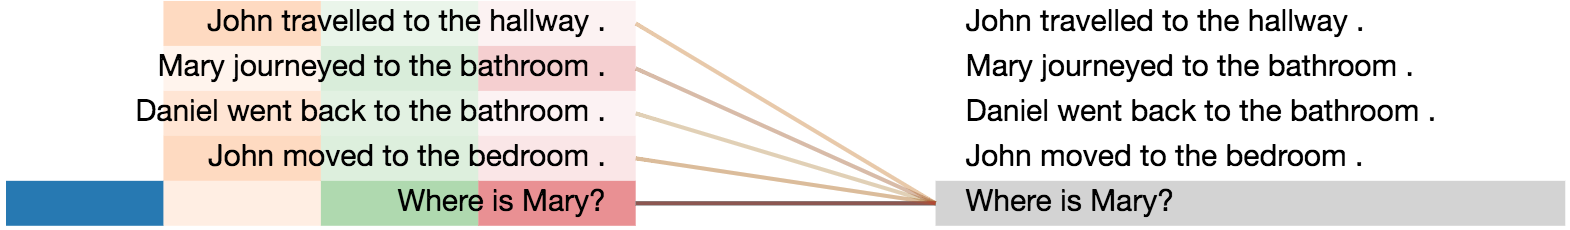
\includegraphics[height=0.8in]{04-part-03/chapter-06/figs_and_tables/figs_attention_babi/e1-step1.png}
        \caption{Step 1}
    \end{subfigure}%
    \hfill \hfill
    \begin{subfigure}[t]{\textwidth}
        \centering
        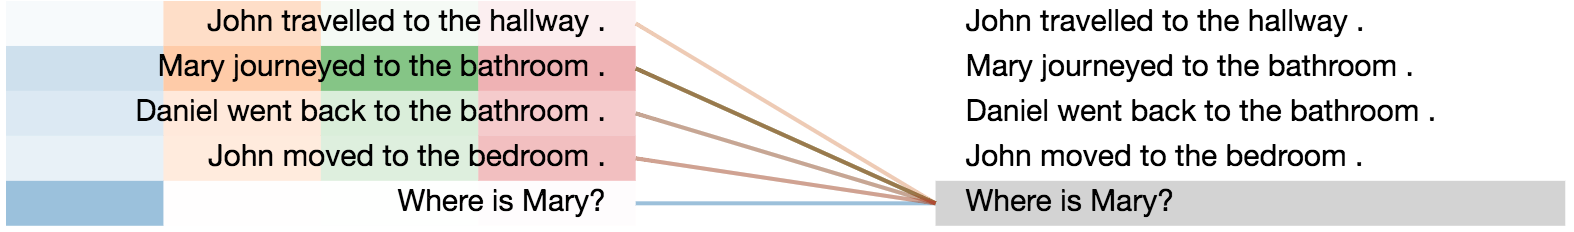
\includegraphics[height=0.8in]{04-part-03/chapter-06/figs_and_tables/figs_attention_babi/e1-step2}
        \caption{Step 2}
    \end{subfigure}
    \hfill \hfill
    \begin{subfigure}[t]{\textwidth}
        \centering
        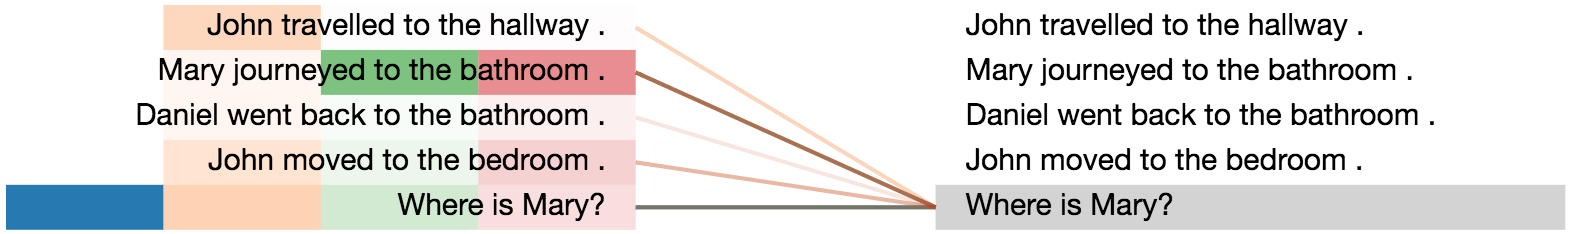
\includegraphics[height=0.8in]{04-part-03/chapter-06/figs_and_tables/figs_attention_babi/e1-step3}
        \caption{Step 3}
    \end{subfigure}
    \hfill \hfill 
    \begin{subfigure}[t]{\textwidth}
        \centering
        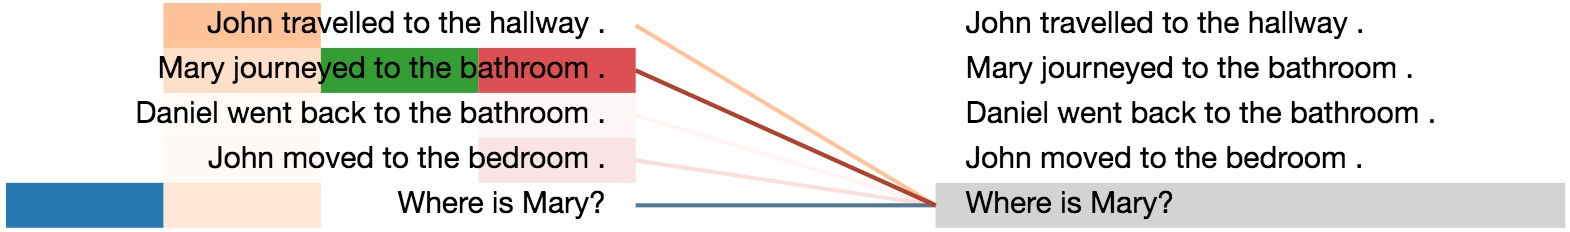
\includegraphics[height=0.8in]{04-part-03/chapter-06/figs_and_tables/figs_attention_babi/e1-step4}
        \caption{Step 4}
    \end{subfigure}
\end{minipage}
    \caption{\label{fig:ex1}Visualization of the attention distributions, when encoding the question: \emph{``Where is Mary?''}.}
\end{figure}
\afterpage{\clearpage}




\begin{figure}[!h]
\begin{minipage}{\textwidth}
\fontsize{8}{8}\fontfamily{pcr}\selectfont
\begin{tabular}{l l}
\textbf{An example from tasks 2}: & \textbf{(requiring two supportive facts to solve)}\\
\\
\textbf{Story}: & \\
& Sandra journeyed to the hallway. \\
& Mary went to the bathroom. \\
& Mary took the apple there. \\
& Mary dropped the apple. \\
\\
\textbf{Question}: & \\
& Where is the apple? \\
\textbf{Model's output}: & \\
& bathroom
\end{tabular}
\end{minipage}
\\  \vfill
\vspace{20pt} % maximize space between the minipages
\begin{minipage}{\textwidth}
    \centering
    \begin{subfigure}[t]{\textwidth}
        \centering
        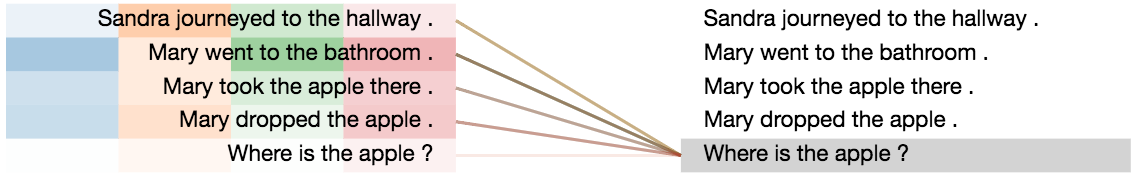
\includegraphics[height=0.8in]{04-part-03/chapter-06/figs_and_tables/figs_attention_babi/e2-step1}
        \caption{Step 1}
    \end{subfigure}%
    \hfill \hfill
    \begin{subfigure}[t]{\textwidth}
        \centering
        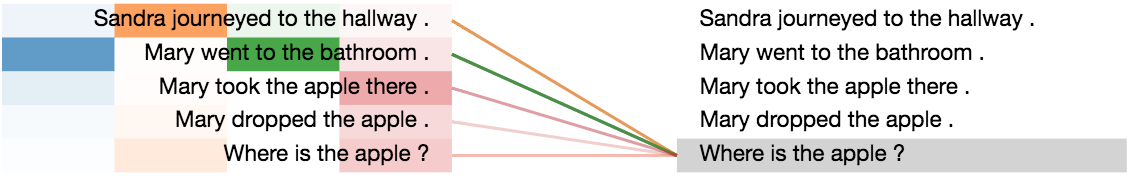
\includegraphics[height=0.8in]{04-part-03/chapter-06/figs_and_tables/figs_attention_babi/e2-step2}
        \caption{Step 2}
    \end{subfigure}
    \hfill \hfill
    \begin{subfigure}[t]{\textwidth}
        \centering
        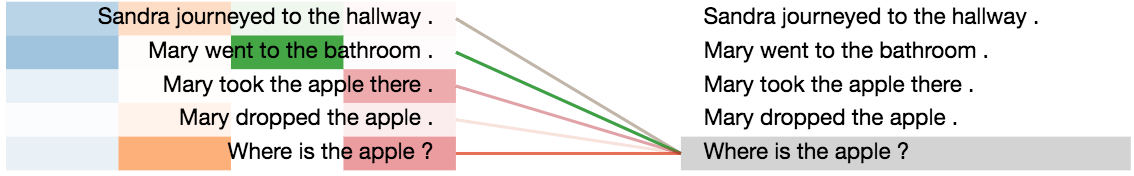
\includegraphics[height=0.8in]{04-part-03/chapter-06/figs_and_tables/figs_attention_babi/e2-step3}
        \caption{Step 3}
    \end{subfigure}
    \hfill \hfill 
    \begin{subfigure}[t]{\textwidth}
        \centering
        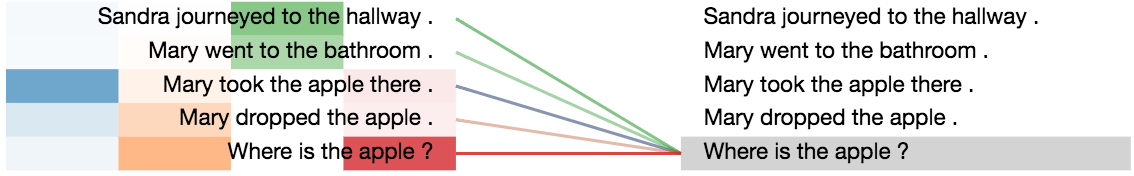
\includegraphics[height=0.8in]{04-part-03/chapter-06/figs_and_tables/figs_attention_babi/e2-step4}
        \caption{Step 4}
    \end{subfigure}
    \end{minipage}
    \caption{\label{fig:ex2}Visualization of the attention distributions, when encoding the question: \emph{``Where is the apple?''}.}
\end{figure}

\afterpage{\clearpage}

\begin{figure}[!h]
\begin{minipage}{\textwidth}
\fontsize{8}{8}\fontfamily{pcr}\selectfont
\begin{tabular}{l l}
\textbf{An example from tasks 2}: & \textbf{(requiring two supportive facts to solve)}\\
\\
\textbf{Story}: & \\
& John went to the hallway. \\
& John went back to the bathroom. \\
& John grabbed the milk there. \\
& Sandra went back to the office. \\
& Sandra journeyed to the kitchen. \\
& Sandra got the apple there. \\
& Sandra dropped the apple there. \\
& John dropped the milk. \\
\\
\textbf{Question}: & \\
& Where is the milk? \\
\textbf{Model's output}: & \\
& bathroom
\end{tabular}
\end{minipage}
\\ \vfill
\vspace{20pt} % maximize space between the minipages
\begin{minipage}{\textwidth}
    \centering
    \begin{subfigure}[t]{\textwidth}
        \centering
        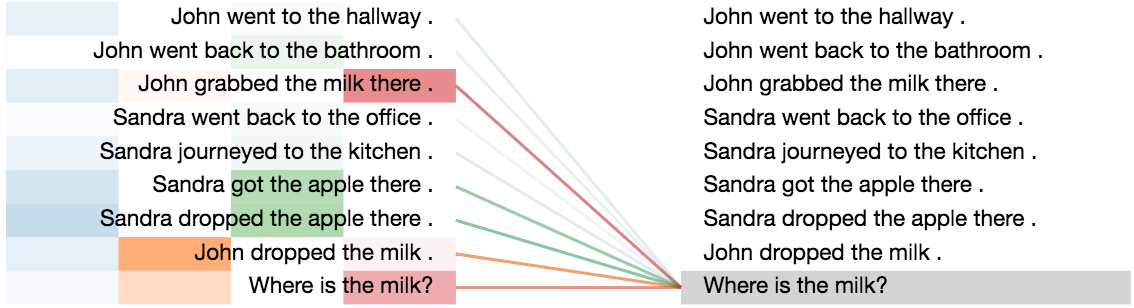
\includegraphics[height=1.3in]{04-part-03/chapter-06/figs_and_tables/figs_attention_babi/e3-step1}
        \caption{Step 1}
    \end{subfigure}%
    \hfill \hfill
    \begin{subfigure}[t]{\textwidth}
        \centering
        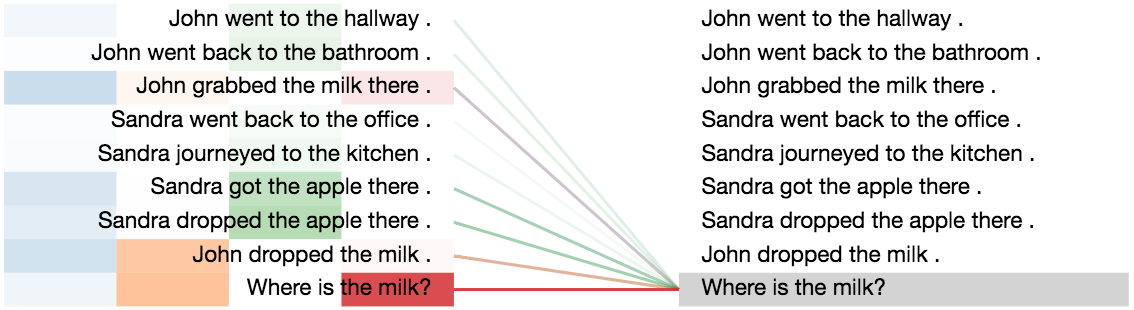
\includegraphics[height=1.3in]{04-part-03/chapter-06/figs_and_tables/figs_attention_babi/e3-step2}
        \caption{Step 2}
    \end{subfigure}
    \hfill \hfill
    \begin{subfigure}[t]{\textwidth}
        \centering
        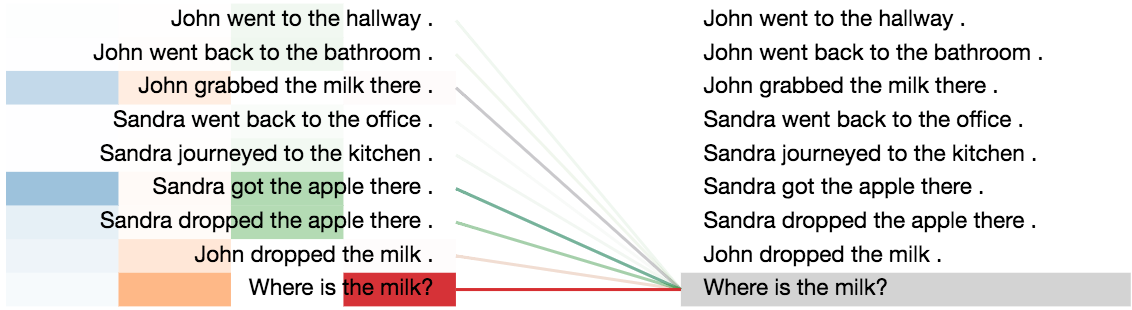
\includegraphics[height=1.3in]{04-part-03/chapter-06/figs_and_tables/figs_attention_babi/e3-step3}
        \caption{Step 3}
    \end{subfigure}
    \hfill \hfill 
    \begin{subfigure}[t]{\textwidth}
        \centering
        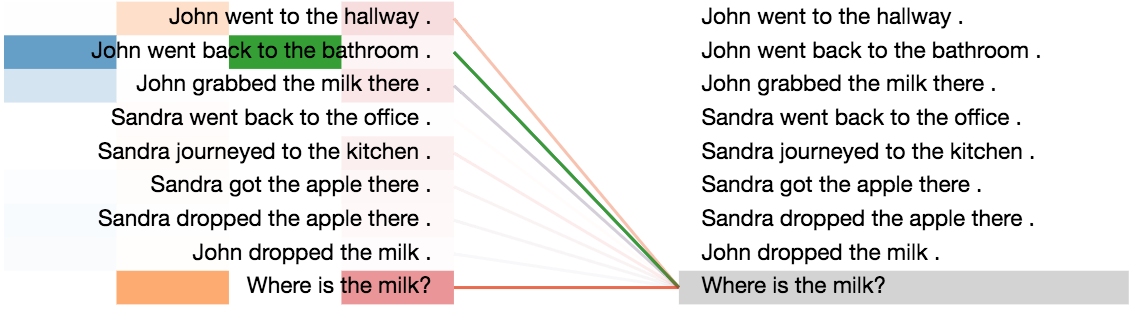
\includegraphics[height=1.3in]{04-part-03/chapter-06/figs_and_tables/figs_attention_babi/e3-step4}
        \caption{Step 4}
    \end{subfigure}
    \end{minipage}
    \caption{\label{fig:ex3}Visualization of the attention distributions, when encoding the question: \emph{``Where is the milk?''}.}
\end{figure}

\afterpage{\clearpage}

\begin{figure}[!h]
\begin{minipage}{\textwidth}
\fontsize{8}{8}\fontfamily{pcr}\selectfont
\begin{tabular}{l l}
\textbf{An example from tasks 3}: & \textbf{(requiring three supportive facts to solve)}\\
\\

\textbf{Story}: & \\
Mary got the milk. \\
& John moved to the bedroom. \\
& Daniel journeyed to the office. \\
& John grabbed the apple there. \\
& John got the football. \\
& John journeyed to the garden. \\
& Mary left the milk. \\
& John left the football. \\
& Daniel moved to the garden. \\
& Daniel grabbed the football. \\
& Mary moved to the hallway. \\
& Mary went to the kitchen. \\
& John put down the apple there. \\
& John picked up the apple. \\
& Sandra moved to the hallway. \\
& Daniel left the football there. \\
& Daniel took the football. \\
& John travelled to the kitchen. \\
& Daniel dropped the football. \\
& John dropped the apple. \\
& John grabbed the apple. \\
& John went to the office. \\
& Sandra went back to the bedroom. \\
& Sandra took the milk. \\
& John journeyed to the bathroom. \\
& John travelled to the office. \\
& Sandra left the milk. \\
& Mary went to the bedroom. \\
& Mary moved to the office. \\
& John travelled to the hallway. \\
& Sandra moved to the garden. \\
& Mary moved to the kitchen. \\
& Daniel took the football. \\
& Mary journeyed to the bedroom. \\
& Mary grabbed the milk there. \\
& Mary discarded the milk. \\
& John went to the garden. \\
& John discarded the apple there. \\
\\
\textbf{Question}: & \\
& Where was the apple before the bathroom? \\
\textbf{Model's output}: & \\
& office
\end{tabular}
\end{minipage}
\end{figure}
\begin{figure}[h!]\ContinuedFloat
\begin{minipage}{\textwidth}
    \centering
    \begin{subfigure}[t]{\textwidth}
        \centering
        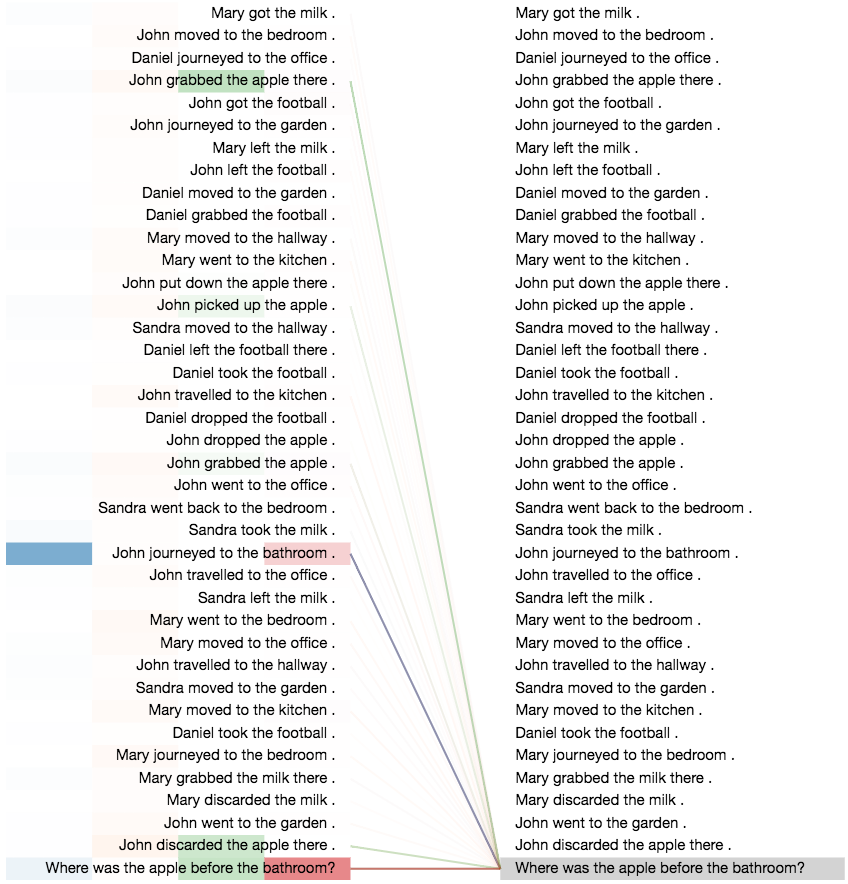
\includegraphics[height=4.2in]{04-part-03/chapter-06/figs_and_tables/figs_attention_babi/e4-step1}
        \caption{Step 1}
    \end{subfigure}%
    \hfill \hfill
    \begin{subfigure}[t]{\textwidth}
        \centering
        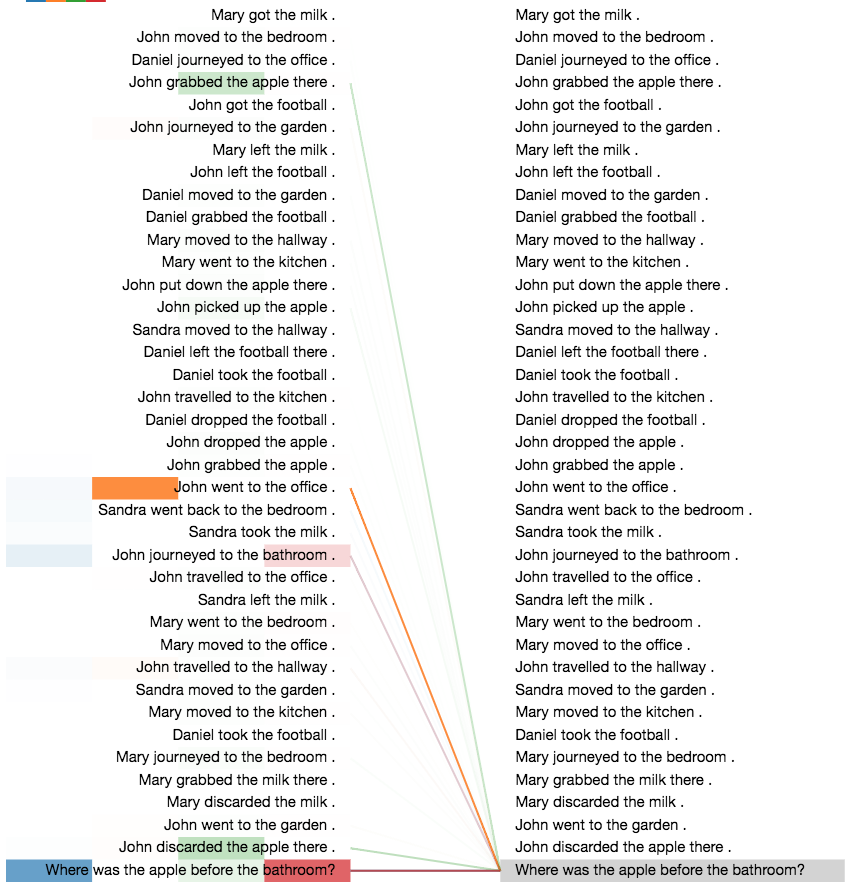
\includegraphics[height=4.2in, trim={0 0 0 0.1cm},clip]{04-part-03/chapter-06/figs_and_tables/figs_attention_babi/e4-step2}
        \caption{Step 2}
    \end{subfigure}
\end{minipage}
\end{figure}
\begin{figure}[h!]\ContinuedFloat
\begin{minipage}{\textwidth}\ContinuedFloat
    \begin{subfigure}[t]{\textwidth}
        \centering
        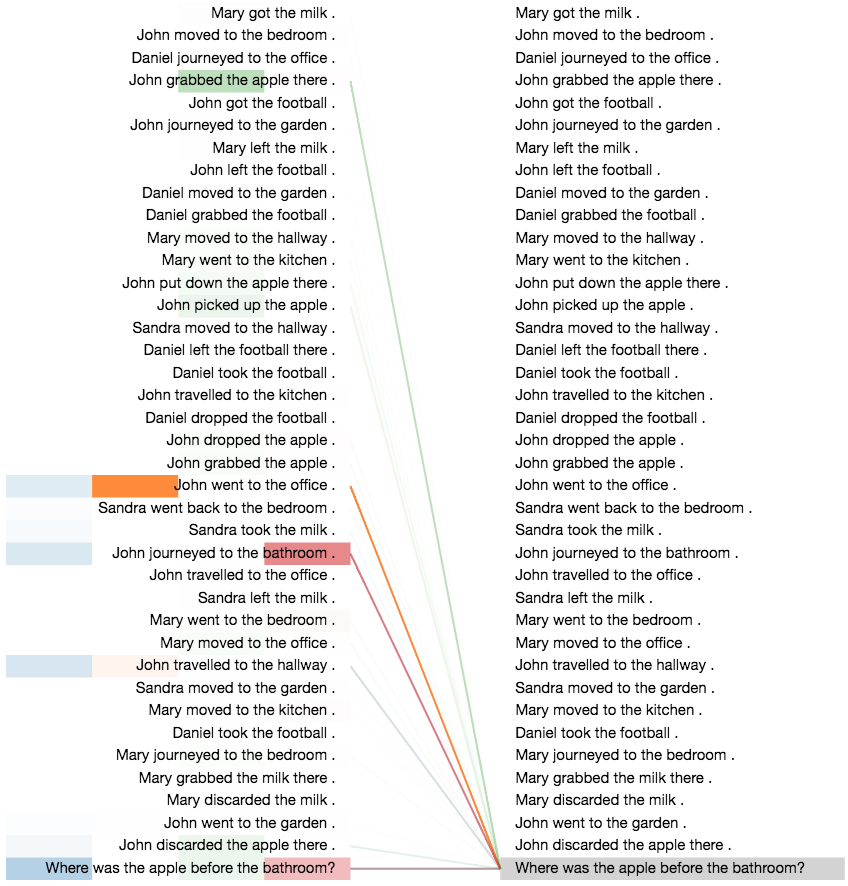
\includegraphics[height=4.2in]{04-part-03/chapter-06/figs_and_tables/figs_attention_babi/e4-step3}
        \caption{Step 3}
    \end{subfigure}
    \hfill \hfill 
    \begin{subfigure}[t]{\textwidth}
        \centering
        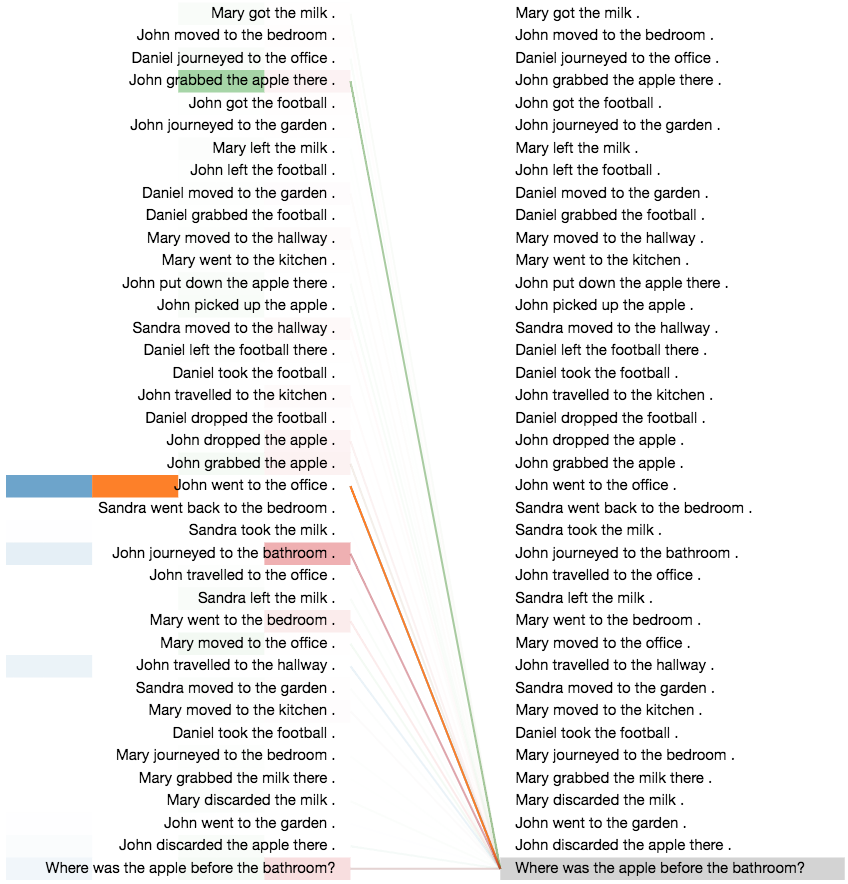
\includegraphics[height=4.2in]{04-part-03/chapter-06/figs_and_tables/figs_attention_babi/e4-step4}
        \caption{Step 4}
    \end{subfigure}
    \caption{\label{fig:ex4}Visualization of the attention distributions, when encoding the question: \emph{``Where was the apple before the bathroom?''}.}
\end{minipage}
\end{figure}

Figures~\ref{fig:ex1}, \ref{fig:ex2}, \ref{fig:ex3}, and \ref{fig:ex4} present visualizations of the attention distributions on bAbI tasks for some examples from Task 1, 2, and 3. The visualization of attention weights is over different time steps based on different heads over all the facts in the story and a question. Different color bars on the left side indicate attention weights based on different heads (4 heads in total).

The above examples illustrate that there is a notion of temporal states in UT, where the model updates its states (memory) in each step based on the output of previous steps, and this chain of updates can also be viewed as steps in a multi-hop reasoning process.

\subsection{Algorithmic Tasks}
The generic neural network architectures cannot generalize well in algorithmic and numerical tasks requiring arithmetic operations such as addition, multiplication etc., even when they may successfully fit any given training data in such tasks, and sometimes they cannot even achieve that~\citep{trask2018neural}. This can be even harder when the distribution of samples' length is different in train and test set.

We trained UTs on three algorithmic tasks, namely Copy, Reverse, and (integer) Addition, all on strings composed of decimal symbols (`0'-`9'). In all the experiments, we train the models on sequences with maximum length of 40 and evaluated on sequences with maximum length of 400~\citep{neural_gpu} to assess the ability of the models on \emph{length generalization}. In fact, the limitation in training data in this task is the lack of coverage over all possible samples (all possible length), not the number of training samples.

As an additional inductive bias for UTs on these tasks, when calculating the positional embedding, we use positions starting with randomized offsets per sample. This way, we further encourage the model to learn position-relative transformations, which improves length generalization.
Results are shown in Table~\ref{tab:algorithmic}. Both UT and UT with randomized position offset outperform LSTM and vanilla Transformer by a wide margin on all three tasks. 
The Neural GPU reports perfect results on this task~\citep{neural_gpu}, however, we note that this result required a special curriculum-based training protocol which was not used for other models.

\begin{table}[t!]
\centering
    \caption{Accuracy (higher better) on the algorithmic tasks. $^*$Note that the Neural GPU was trained with a special curriculum to obtain the perfect result, while other models are trained without any curriculum.}
    \label{tab:algorithmic}
    \begin{adjustbox}{max width=\textwidth}
    \begin{tabular}{lcccccc}
        & & & & & & \\ \toprule
        \multirow{2}{*}{ \bf Model } & \multicolumn{2}{c}{ \textbf{Copy} } & \multicolumn{2}{c}{ \textbf{Reverse} } & \multicolumn{2}{c}{ \textbf{Addition} } \\ \cmidrule(l{2pt}r{2pt}){2-3} \cmidrule(l{2pt}r{2pt}){4-5} \cmidrule(l{2pt}r{2pt}){6-7}
        & \textit{char-acc} & \textit{seq-acc} & \textit{char-acc} & \textit{seq-acc} & \textit{char-acc} & \textit{seq-acc} \\ \midrule
        \bf LSTM & 0.45 & 0.09 & 0.66 & 0.11 & 0.08 & 0.0 \\
        \bf Transformer & 0.53 & 0.03 & 0.13 & 0.06 & 0.07 & 0.0 \\
        \bf Universal Transformer & 0.76 & 0.29 & 0.83 & 0.41 & 0.32 & 0.02 \\
        \bf UT w/ randomized offset & 0.91 & 0.35 & 0.96 & 0.46 & 0.34 & 0.02 \\
        \bf Neural GPU$^*$ & \textbf{1.00} & \textbf{1.00} & \textbf{1.00} & \textbf{1.00} & \textbf{1.00} &
        \textbf{1.00} \\ \bottomrule
    \end{tabular}
    \end{adjustbox}
\end{table}

\subsection{Learning to Execute (LTE)}
As another class of sequence-to-sequence learning problems, we also evaluate UTs on Learning to Execute (LTE) tasks. 
LTE is a set of tasks indicating the ability of a model to learn to execute computer programs and was proposed by~\citet{ZS14}. These tasks include two subsets: 1) program evaluation tasks (program, control, and addition) that are designed to assess the ability of models for understanding numerical operations, if-statements, variable assignments, the compositionality of operations, and more, as well as 2) memorization tasks (copy, double, and reverse). 

The difficulty of the program evaluation tasks is parameterized by their \textit{length} and \textit{nesting}. The
length parameter is the number of digits in the integers that appear in the programs (so the integers are chosen uniformly from [1, \emph{length}]), and the nesting parameter is the number of times we are allowed to combine the operations with each
other. Higher values of nesting yield programs with deeper parse trees.
For instance, here is a program that is generated with length = 4 and
nesting = 3. 
\begin{table}[h!]
\fontsize{8}{8}\fontfamily{pcr}\selectfont
\begin{tabular}{l l}
\textbf{Input}: & \\
& j=8584 \\
& {\color{blue}{for}} x {\color{blue}{in}} range(8): \\
& ~~j+=920 \\
& b=(1500+j) \\
& {\color{blue}{print}}((b+7567)) \\
\textbf{Target}: & \\
& 25011
\end{tabular}
\end{table}

\begin{table}[t!]
    \centering
    \caption{Character-level (\emph{char-acc}) and sequence-level accuracy (\emph{seq-acc}) results on the Memorization LTE tasks, with maximum length of 55.}
    \label{tab:lte-mem}
    \begin{adjustbox}{max width=\textwidth}
    \begin{tabular}{lcccccc}
        \toprule
        %& \multicolumn{7}{c}{Memorization Tasks} \\
        & \multicolumn{2}{c}{ \bf Copy } & \multicolumn{2}{c}{ \bf Double } & \multicolumn{2}{c}{ \bf Reverse } \\
        \cmidrule(l{2pt}r{2pt}){2-3} \cmidrule(l{2pt}r{2pt}){4-5} \cmidrule(l{2pt}r{2pt}){6-7}
        \bf Model & \textit{char-acc} & \textit{seq-acc} & \textit{char-acc} & \textit{seq-acc} & \textit{char-acc} & \textit{seq-acc} \\ \midrule
        \bf LSTM & 0.78 & 0.11 & 0.51 & 0.05 & 0.91 & 0.32 \\
        \bf Transformer & 0.98 & 0.63 & 0.94 & 0.55 & 0.81 & 0.26 \\
        \bf Universal Transformer & \textbf{1.00} & \textbf{1.00} & \textbf{1.00} & \textbf{1.00} & \textbf{1.00} & \textbf{1.00} \\ \bottomrule
    \end{tabular}
    \end{adjustbox}
\end{table}

\begin{table}[t!]
    \centering
    \caption{Character-level (\emph{char-acc}) and sequence-level accuracy (\emph{seq-acc}) results on the Program Evaluation LTE tasks with maximum nesting of 2 and length of 5.}
    \label{tab:lte-prog}
    \begin{adjustbox}{max width=\textwidth}
    \begin{tabular}{lcccccc}
    \toprule
        & \multicolumn{2}{c}{ \bf Program } & \multicolumn{2}{c}{ \bf Control } & \multicolumn{2}{c}{ \bf Addition } \\ \cmidrule(l{2pt}r{2pt}){2-3} \cmidrule(l{2pt}r{2pt}){4-5} \cmidrule(l{2pt}r{2pt}){6-7}
        \bf Model & \textit{char-acc} & \textit{seq-acc} & \textit{char-acc} & \textit{seq-acc} & \textit{char-acc} & \textit{seq-acc} \\ \midrule
        \bf LSTM & 0.53 & 0.12 & 0.68 & 0.21 & 0.83 & 0.11 \\
        \bf Transformer & 0.71 & 0.29 & 0.93 & 0.66 & \textbf{1.00} & \textbf{1.00} \\
        \bf Universal Transformer & \textbf{0.89} & \textbf{0.63} & \textbf{1.00} & \textbf{1.00} & \textbf{1.00} & \textbf{1.00} \\
    \bottomrule
    \end{tabular}
    \end{adjustbox}
\end{table}

We use the mix-strategy discussed in~\citep{ZS14} to generate the datasets. Unlike~\citep{ZS14}, we do not use any curriculum learning strategy during training and we make no use of target sequences at test time. Tables~\ref{tab:lte-mem} and \ref{tab:lte-prog} present the performance of an LSTM model, Transformer, and Universal Transformer on the program evaluation and memorization tasks, respectively. UT achieves perfect scores in all the memorization tasks and also outperforms both LSTMs and Transformers in all program evaluation tasks by a wide margin. 


\subsection{Subject-Verb Agreement}
Next, we consider the task of predicting number-agreement between subjects and verbs in English sentences~\citep{linzen2016assessing}. Succeeding in this task is a strong indicator that a model can learn to approximate syntactic structure and therefore it was proposed by~\citet{linzen2016assessing} as a proxy for assessing the ability of different models to capture hierarchical structure in natural language. 

Two experimental setups were proposed by ~\citet{linzen2016assessing} for training a model on this task: 1) training with a language modeling objective, i.e., next word prediction, and 2) as binary classification, i.e., predicting the number of the verb given the sentence. 
We follow the experimental protocol of ~\citet{linzen2016assessing} for solving the task using a language modeling training setup, i.e., a next word prediction objective, followed by calculating the ranking accuracy of the target verb at test time. 

In this task, in order to have different levels of difficulty, ``agreement attractors'' are used, i.e., one or more intervening nouns with the opposite number from the subject with the goal of confusing the model. In this case, the model needs to correctly identify the head of the syntactic subject that corresponds to a given verb and ignore the intervening attractors in order to predict the correct form of that verb.
Here are some examples for this task in which subjects and the corresponding verbs are in boldface and agreement attractors are underlined:
\begin{table}[h!]
\fontsize{9}{10}\fontfamily{pcr}\selectfont
\begin{tabular}{l l}
\textbf{No attractor:} & The \textbf{boy} \textbf{smiles}. \\
\textbf{One attractor:}  &  The \textbf{number} of \underline{men} \textbf{is} not clear. \\
\textbf{Two attractors:}  &  The \textbf{ratio} of \underline{men} to \underline{women} \textbf{is} not clear. \\
\textbf{Three attractors:} &  The \textbf{ratio} of \underline{men} to \underline{women} and \underline{children} \textbf{is} not clear. 
\end{tabular}
\end{table}

\begin{table}
\centering
\begin{adjustbox}{max width=\textwidth}
\begin{tabular}{lccccccc}
\toprule
\multirow{2}{*}{ \bf Model } & \multicolumn{6}{c}{ \bf Number of attractors } & \\ \cmidrule{2-7}
& \textit{0} & \textit{1} & \textit{2} & \textit{3} & \textit{4} & \textit{5} & \textit{Total} \\ \midrule
\multicolumn{8}{c}{ \bf Previous best results~\citep{yogatama2018memory}: } \\ \midrule
\bf Best Stack-RNN & \emph{0.994} & 0.979 & 0.965 & 0.935 & 0.916 & 0.880 & 0.992 \\
\bf Best LSTM & 0.993 & 0.972 & 0.950 & 0.922 & 0.900 & 0.842 & 0.991 \\
\bf Best Attention & \textbf{0.994} & \textbf{0.977} & 0.959 & 0.929 & 0.907 & 0.842 & \textbf{0.992} \\ \midrule
\multicolumn{8}{c}{ \bf Our results: } \\ \midrule
\bf Transformer & 0.973 & 0.941 & 0.932 & 0.917 & 0.901 & 0.883 & 0.962 \\
\bf Universal Transformer & 0.993 & 0.971 & \textbf{0.969} & 0.940 & 0.921 & 0.892 & \textbf{0.992} \\
\bf UT w/ ACT & \textbf{0.994}	& 0.969	& 0.967	& \textbf{0.944}	& \textbf{0.932}	& \textbf{0.907}	& \textbf{0.992} \\
\midrule
\bf $\Delta$ (UT w/ ACT - Best) & 0 & -0.008 & 0.002 & 0.009 & 0.016 & 0.027 & - \\
 \bottomrule
\end{tabular}
\end{adjustbox}
\caption{Accuracy on the subject-verb agreement number prediction task (higher is better).}
\label{tab:sva}
\end{table}
Our results are summarized in Table~\ref{tab:sva}. The best LSTM with attention from the literature achieves 99.18\% on this task~\citep{yogatama2018memory}, outperforming a vanilla Transformer~\citep{tran18}. UTs significantly outperform standard Transformers, and achieve an \emph{average} result comparable to the current state of the art (99.2\%). However, we see that UTs (and particularly with dynamic halting) perform progressively better than all other models as the number of attractors increases (see the last row, $\Delta$).
The recurrent inductive bias, i.e., the fact that we can repeat the computations in depth, helps the Universal Transformer to capture the hierarchical relations and better model the structure of the data.

\subsection{LAMBADA Language Modeling}
The LAMBADA task~\citep{paperno2016lambada} is a language modeling task consisting of predicting a missing target word given a broader context of 4-5 preceding sentences. The dataset was specifically designed so that humans are able to accurately predict the target word when shown the full context, but not when only shown the target sentence in which it appears. It, therefore, goes beyond language modeling, and tests the ability of a model to incorporate broader discourse and longer term context when predicting the target word\footnote{\url{http://clic.cimec.unitn.it/lambada/appendix_onefile.pdf}}.
Here is a sample from the dataset:

\begin{table}[h!]
\fontsize{8}{10}\fontfamily{pcr}\selectfont
\begin{tabular}{l l}
\textbf{Context}: & \\
& ``Yes, I thought I was going to lose the baby.'' \\
&  ``I was scared too,'' he stated, sincerity flooding his eyes. \\ 
&  ``You were?'' ``Yes, of course. Why do you even ask?''  \\
&  ``This baby wasn't exactly planned for.''
\\
\textbf{Target sentence}: & \\
& ``Do you honestly think that I would want you to have a \_\_\_\_\_\_\_\_?'' 
\\
\textbf{Target word}:  & \\  
& miscarriage
\end{tabular}
\end{table}

The LAMBADA task consists in predicting the target word given the whole passage (i.e., the context plus the target sentence). A ``control set''  is also provided which was constructed by randomly sampling passages of the same shape and size as the ones used to build LAMBADA, but without filtering them in any way. The control set is used to evaluate the models at standard language modeling before testing on the LAMBADA task, and therefore to ensure that low performance on the latter cannot be attributed simply to poor language modeling.

The task is evaluated in two settings: as \emph{language modeling} (the standard setup) and as \emph{reading comprehension}. In the former (more challenging) case, a model is simply trained for the next-word prediction on the training data, and evaluated on the target words at test time (i.e., the model is trained to predict all words, not specifically challenging target words).  In the latter setting, introduced by Chu et al.~\cite{chu2017broad}, the target sentence (minus the last word) is used as the query for selecting the target word from the context sentences. Note that the target word appears in the context 81\% of the time, making this setup much simpler. However, the task is impossible in the remaining 19\% of the cases.

\begin{table}[t!]
\centering
    \begin{adjustbox}{max width=\textwidth}
    \begin{tabular}{lcccccc}
    \toprule
    \multirow{2}{*}{ \bf Model } & \multicolumn{3}{c}{\bf LM Perplexity \& (Accuracy) } & \multicolumn{3}{c}{\bf RC Accuracy } \\ \cmidrule(l{2pt}r{2pt}){2-4} \cmidrule(l{2pt}r{2pt}){5-7}
    & \textit{control} & \textit{dev} & \textit{test} & \textit{control} & \textit{dev} & \textit{test} \\ \midrule
    \bf Neural Cache~\citep{grave2016improving} & {\bf 129} & 139 & - & - & - & - \\ 
    \bf Dhingra et al.~\cite{dhingra2018neural} & - & - & - & - & - & 0.5569 \\ \midrule
    \bf Transformer & 142 (0.19) & 5122 (0.0) & 7321 (0.0) & 
    0.4102 & 0.4401 & 0.3988 \\
    \bf LSTM & 138 (0.23) & 4966 (0.0) & 5174 (0.0) & 0.1103 & 0.2316 & 0.2007 \\
    \bf UT \emph{base}, 6 steps (fixed) & 131 (0.32) & 279 (0.18) & 319 (0.17) & {\bf 0.4801} & 0.5422 & 0.5216 \\
    \bf UT w/ dynamic halting & 130 (0.32) & {\bf 134} (0.22) & {\bf 142} (0.19) & 0.4603 & {\bf 0.5831} & {\bf 0.5625} \\ \midrule
    \bf UT \emph{base}, 8 steps (fixed) & 129(0.32) & 192 (0.21) & 202 (0.18) & - & - & - \\
    \bf UT \emph{base}, 9 steps (fixed) & \textbf{129(0.33)} & 214 (0.21) & 239 (0.17) & - & - & - \\
 \bottomrule
    \end{tabular}
    \end{adjustbox}
    \caption{LAMBADA language modeling (LM) perplexity (lower better) with accuracy in parentheses (higher better), and Reading Comprehension (RC) accuracy results (higher better). `-' indicates no reported results in that setting.}
    \label{tab:lambada}
\end{table}

The results are shown in Table~\ref{tab:lambada}. Universal Transformer achieves state-of-the-art results in both the language modeling and reading comprehension setup, outperforming both LSTMs and vanilla Transformers. Note that achieving good results on the control set only shows a model's strength in standard language modeling.

Our best fixed UT results used 6 steps. However, the average number of steps that the best UT with dynamic halting took on the test data over all positions and samples was $8.2 \rpm 2.1$. In order to see if the dynamic model did better simply because it took more steps, we trained two fixed UT models with 8 and 9 steps respectively (see last two rows). Interestingly, these two models achieve better results compared to the model with 6 steps, but \emph{do not outperform the UT with dynamic halting}. This leads us to believe that dynamic halting may act as a useful regularizer for the model via incentivizing smaller numbers of steps for some of the input symbols, while allowing more computation for others.

\subsection{Machine Translation}
We trained a UT on the WMT 2014 English-German translation task using the same setup as reported in \citep{transformer} in order to evaluate its performance on a large-scale sequence-to-sequence task. Results are summarized in Table~\ref{tab:wmt}. The UT with a fully-connected recurrent transition function (instead of separable convolution) and without ACT improves by 0.9 BLEU over a Transformer and 0.5 BLEU over a Weighted Transformer with approximately the same number of parameters \citep{ahmed2017weighted}.

\begin{table}[t!]
    \centering
    \caption{Machine translation results on the WMT14 En-De translation task trained on 8xP100 GPUs in comparable training setups. All \emph{base} results have the same number of parameters.}
    \begin{tabular}{lc}
        \toprule
        \bf{Model} & \bf{BLEU} \\
        \midrule
        \bf Universal Transformer \emph{small} & 26.8 \\
        \bf Transformer \emph{base}~\citep{transformer} & 28.0 \\
        \bf Weighted Transformer \emph{base}~\citep{ahmed2017weighted} & 28.4 \\
       \bf  Universal Transformer \emph{base} & \bf{28.9} \\
        % \midrule
        % Transformer \emph{big}~\citep{transformer} & ??.? \\
        % Universal Transformer \emph{big} & \bf{??.?} \\
        \bottomrule
    \end{tabular}
    \label{tab:wmt}
\end{table}

\subsection{Open-Domain Question Answering}
Open-domain question answering aims to satisfy users who are looking for a direct answer to a complex information need. 
This requires querying large open-domain knowledge sources like the Web. 
Inferring the answer to a question given multiple documents that potentially contain the answer, is at the heart of the open-domain question answering task. 
Most open-domain question answering systems described in the literature first retrieve relevant documents or passages, select one or a few of them as the context, and then feed the question and the context to a reading comprehension system to extract the answer~\citep{buck2017ask, chen2017reading, seo2016bidirectional, dhingra2016gated}. 
However, the information needed to answer complex questions is not always contained in a single, directly relevant document that is ranked high. In many cases, there is a need to read multiple documents, combine them, and reason over the facts from these documents to be able to give the correct answer to the question.

For example, in Figure~\ref{fig:example}, in order to infer the correct answer to the question: ``\texttt{Who is the Spanish artist, sculptor and draughtsman famous for co-founding the Cubist movement?}'' given the top-ranked document, a reading comprehension system most likely will extract ``\texttt{Georges Braque}'' as the answer, which is not the correct answer. 
In this example, in order to infer the correct answer, one has to go down the ranked list, gather and encode facts, even those that are not immediately relevant to the question, like ``\emph{Malaga is a city in Spain},'' which can be inferred from a document at rank 66, and then in a multi-step reasoning process, infer some new facts, including ``\emph{Picasso was a Spanish artist}'' given documents at ranks~12 and~66, and ``\emph{Picasso, who was a Spanish artist, co-founded the Cubist}'' given the previously inferred fact and the document ranked third. 

\begin{figure}[!t]
 \centering
 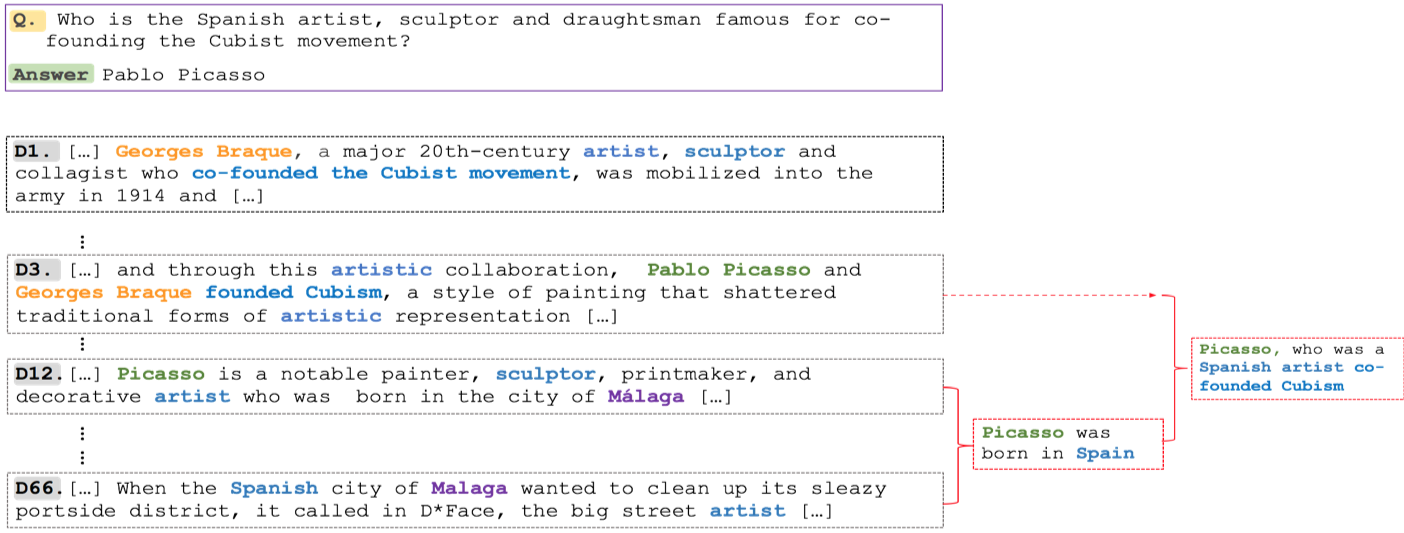
\includegraphics[width=\textwidth]{04-part-03/chapter-06/figs_and_tables/fig_od_example.png}
%  \vspace{1pt}
 \caption{Example complex question answering that requires that information from multiple documents be combined and some amount of reasoning over the information extracted from those documents. (Best viewed in color.)}
 \label{fig:example}
\end{figure}

In this example, and in general in many cases in open-domain question answering, a piece of information in a low-ranked document that is not immediately relevant to the question, may be useful to fill in the blanks and complete information extracted from the top relevant documents and eventually support inferring the correct answer.
However, most open-domain question answering methods focus on only one or a few candidate documents by filtering out the less relevant documents to avoid dealing with noisy information and operate over the selected set of documents to extract the answer~\citep{wang2017r, wang2017evidence,lin2018denoising}. 

We propose a new architecture, called \tracrnet (pronounced \emph{Tracker Net}, that combines Transformer and  Universal Transformer to improve open-domain question answering by explicitly operating on a larger set of candidate documents during the whole question answering process and learning how to aggregate and reason over information from these documents in an effective way while trying not to be distracted by noisy documents. 
% 
Given the candidate documents and the question, to generate the answer, \tracrnet first \underline{\textbf{Tra}}nsforms them into vectors by applying a stack of  Transformer blocks with self-attention over words in each document in a layer called \emph{Input Encoding}. 
Then, it updates the learned representations from the first stage by \underline{\textbf{C}}ombining and enriching them through a multihop \underline{\textbf{R}}easoning process by applying multiple steps of the Universal Transformer in a layer called \emph{Multihop Reasoning}.  

% paragraph might be too verbose
Returning to the example in Figure~\ref{fig:example}, after learning representations for each top-ranked document and the question, \tracrnet updates them by applying multiple steps of the Universal Transformer. 
Given the self-attention mechanism and inductive bias of the Universal Transformer, in the first step, \tracrnet can update the representation of document D\#12 by attending to D\#66 (as they are related by both mentioning Malaga) and augment the information in D\#12 with the fact that ``Malaga is city in Spain,'' so the updated vector of D\#12 has the fact that ``Picasso is a Spanish artist'' encoded in itself. 
Then, in the next step of reasoning, \tracrnet can update the representation of D\#3 by attending over the vector representing D\#12 estimated in the previous step, and enrich the information in D\#3 with the fact that ``Picasso is a Spanish artist,'' and the updated vector of D\#3 has the fact that ``Picasso, who was a Spanish artist co-founded Cubism'' encoded in it. 
After that, during answer generation, the decoder can attend to the final vector representing D\#3 and give the correct answer.

% why \tracrnet rocks:
% 1. fast
\tracrnet has a number of desirable features.
%
First, all the building blocks of \tracrnet are based on self-attentive feed-forward neural networks, hence per-symbol hidden state transformations are fully parallelizable, which leads to an enormous speedup during training and a super fast input encoding during inference time compared to RNN based models. 
% 3. It can reason
Second, while there is no recurrence in time in our model, the recurrence in depth in the Universal Transformer used in the \emph{Multihop Reasoning} layer, adds the inductive bias to the model that is needed to go beyond understanding each document separately and combine their information in multiple steps.
% 2. global receptive field -> long docs, a large set of docs
Third, \tracrnet has the global receptive field of the Transformer based models~\citep{vaswani2017attention,Dehghani:ICLR:2019}, which helps it to better encode a long document during \emph{Input Encoding} as well as perform better inference over a rather large set of documents during \emph{Multihop Reasoning}.
% 4. robustness against noise
And fourth, the hierarchical usage of a self-attention mechanism, first over words and then over documents, helps \tracrnet to control its attention both at word and document levels, making it less fragile to noisy input, which is of key importance while encoding many documents.
%
All these properties of \tracrnet come together and lead to an effective and efficient architecture for open-domain question answering. 

We employ \tracrnet on two public open-domain question answering datasets, SearchQA and Quasar-T, and achieve results that meet or exceed the state-of-the-art. 

\subsubsection{\tracrnet} % : Transform, Combine, and Reason}
\label{sec:tra}
In the setup we consider here, the model is given a question $q$ and a set of $n$ relevant documents $C_q=\{D^q_1, D^q_2, \ldots D^q_n\}$ retrieved from the web using a search engine as the input, and the goal is to ``generate'' the answer $a_q$ to the question $q$ based on the supporting document(s) in the set $C_q$.

This is different from the standard Reading Comprehension (RC) tasks~\cite{hermann2015teaching,xiong2016dynamic}. 
First of all, in RC a single document (passage) is given, from which the answer should be extracted. 
Secondly, in RC, a strong supervision on the positions of the answer spans is available during training.
We also assume that the utilized information or techniques to retrieve relevant documents are not available to the model, therefore there is no leverage for getting better-supporting documents.

\begin{figure}[!t]
 \centering
 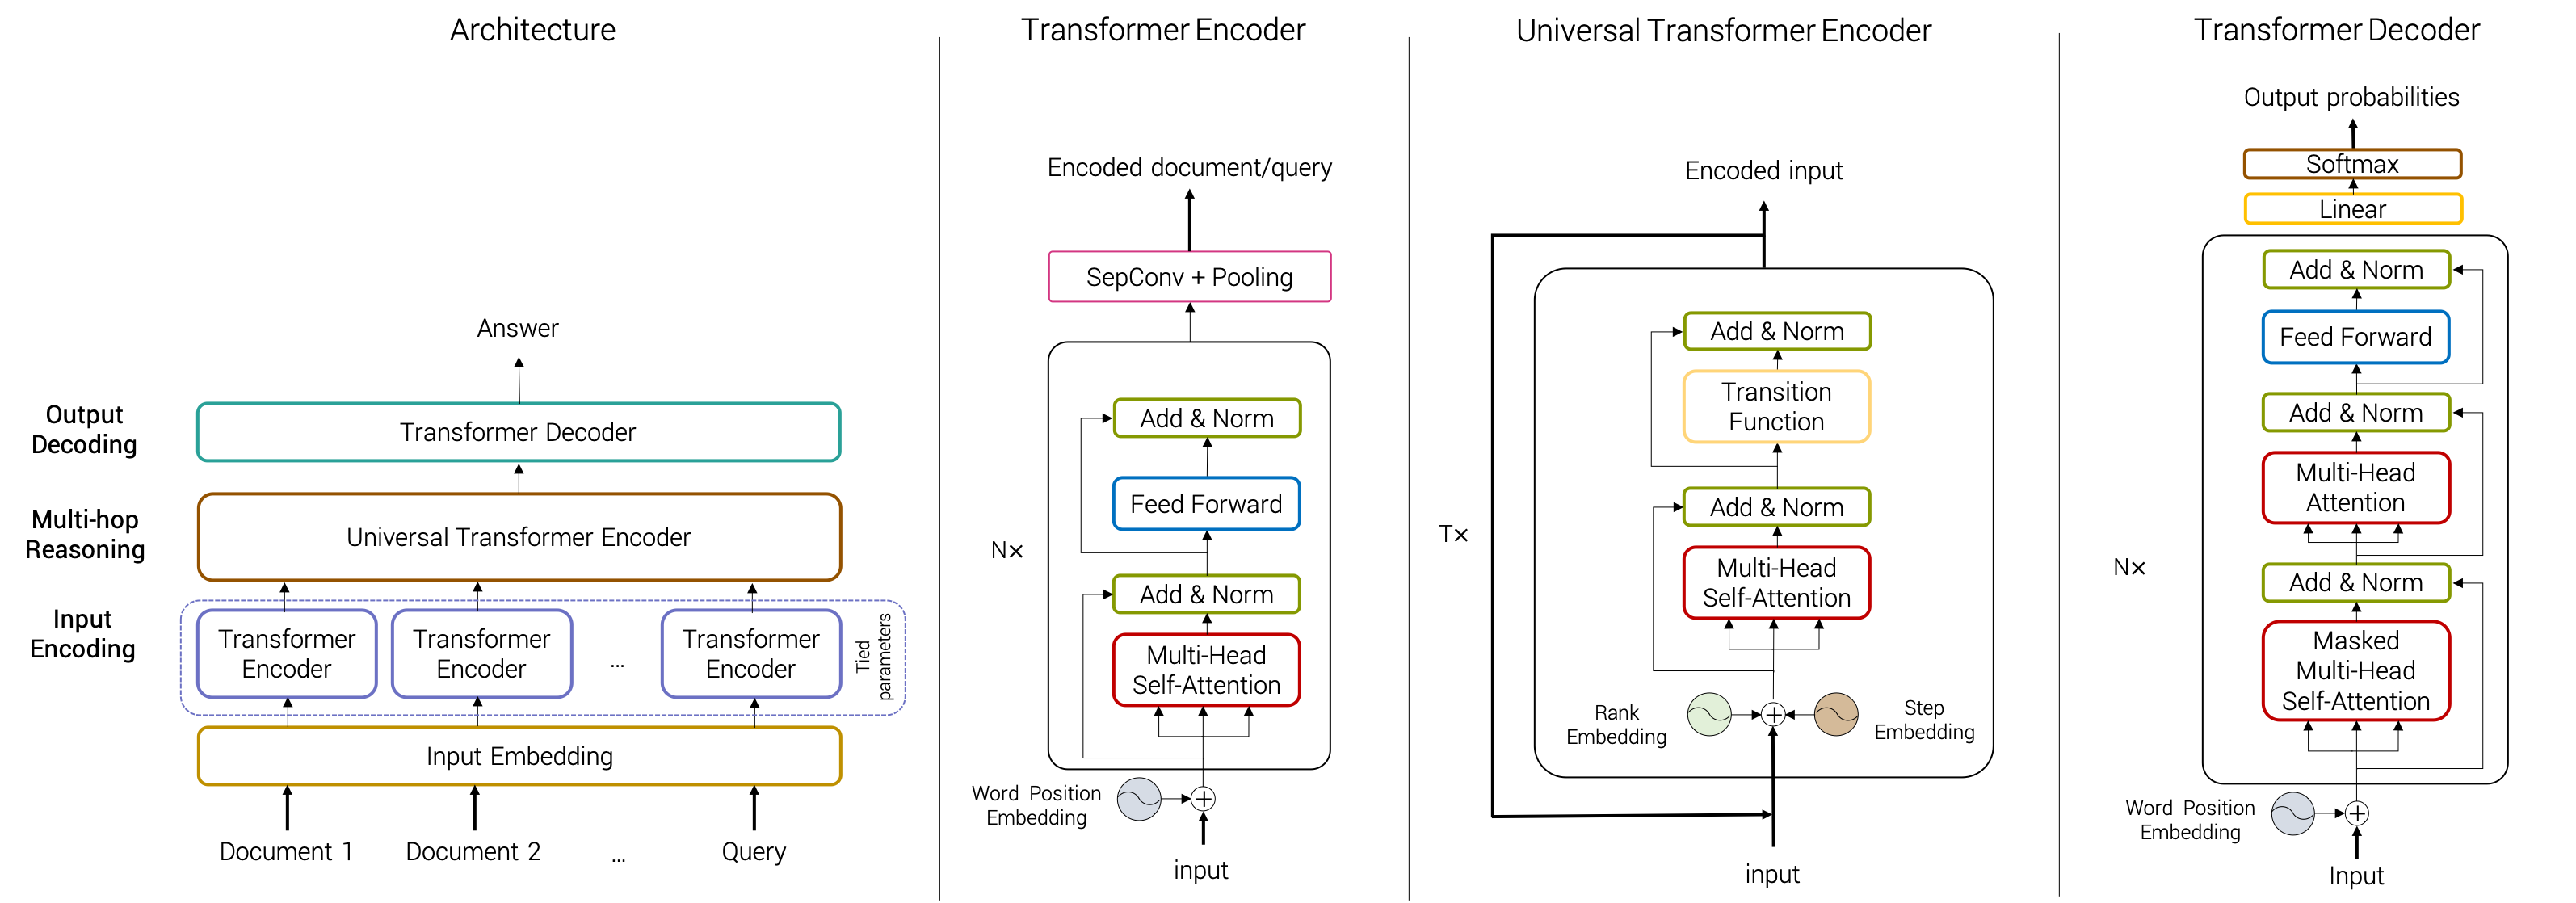
\includegraphics[width=\textwidth]{04-part-03/chapter-06/figs_and_tables/fig_tracrnet.png}
 \caption{An overview of the \tracrnet architecture.}
 \label{fig:model_tracrnet}
\end{figure}

\tracrnet is based on the encoder-decoder architecture, where we have a hierarchy of transformer-based models in the encoder, where the model can attend first over words and then over documents~\citep{Dehghani2017:CIKM}. At the bottom, in the \emph{Input Encoding} layer, we encode each document in $C_q$ as well as the question with transformer blocks with tied parameters that are fed by word-level embeddings. 
Then, we feed the encoded documents and the question from this layer to the \emph{Multihop Reasoning} layer which is, in fact, a universal transformer block where representations of all documents and the question get iteratively updated using multiple steps of self-attention.
Then, we use a stack of transformer decoder blocks as the \emph{Output Decoder} layer to generate the answer. 
%
The general schema of \tracrnet is depicted in Figure~\ref{fig:model_tracrnet}. 
Below, we explain the details of each of these layers in the model.

\mypar{Input encoding} 
The Input Encoding layer is in charge of encoding each of the documents and the question to single vectors given their words' embeddings. For this layer, we used a stack of $N$ Transformer Encoder blocks that is followed by a depth-wise separable convolution~\citep{kaiser2017depthwise,chollet2017xception} and then a pooling function to get a single vector representation for the whole document or the question  (see the \texttt{Transformer Encoder} in Figure~\ref{fig:model_tracrnet}). 
Depth-wise separable convolution is defined by a convolution on each of the feature channels separately, followed by a point-wise convolution that is applied to project them to a feature vector with the desirable depth (see \citep{chollet2017xception} for more details).

\mypar{Multihop reasoning} 
Multihop Reasoning is the layer in which the Universal Transformer is employed to combine evidence from all documents with respect to the question within a multi-step process with the capacity of multihop reasoning.
%
In \tracrnet, the input of the Universal Transformer Encoder is the set of vectors each representing a document in $C_q$ or the question, that are computed by the \emph{Input Encoding} layer  (see  the \texttt{Universal Transformer Encoder} in Figure~\ref{fig:model_tracrnet}). 

In each step of the Universal Transformer, given $H_{t} \in \mathbb{R}^{(|C_q|+1) \times d}$ and the dimension $d$ of the input vectors, we add two embeddings to $H^{t}$: a \emph{Rank Embedding} that encodes the rank of documents given by the retrieval system, also used to distinguish the question from documents (similar to the positional embedding in token level inputs) and the \emph{Step Embedding}. We use Equation\ref{eqn:coordinate-embeddings} to calculate these embeddings.
In our experiments, we use depthwise separable convolution~\cite{chollet2017xception} as the Transition($\cdot$) function.

In the multihop reasoning layer, the representations of all the documents and question learned from the previous layer get updated during $T$ steps of iterating over the Universal Transformer Encode block. 
Self-attention in this layer allows the model to understand each of the documents based on the information in all the documents as well as the question.
In addition, the depth-wise recurrency in the Universal Transformer establishes connections among documents at each step and lays the ground for performing multihop reasoning to solve cases similar to what we have shown in Example~\ref{fig:example}.

\mypar{Output decoder} 
After $T$ steps of refining the representations of documents and the question in the Universal Transformer Encoder, the final output is a matrix of $d$-dimensional vector representations $H \in \mathbb{R}^{(|C_q|+1) \times d}$ for all the documents in $C_q$ and the question $q$.

Given this, we use a stack of $N$ Transformer Decoder blocks (see  the \texttt{Transformer Decoder} in Figure~\ref{fig:model_tracrnet}) to decode the answer.
To generate answers from the model at inference time, we run the model autoregresively~\citep{graves2013generating}, where the model consumes the previously generated symbols at each time step in order to generate the distribution over the vocabulary for the next symbol. From this distribution, we select the symbol with the highest probability as the next symbol.   


\subsubsection{Datasets}
We have conducted experiments on two publicly available open-domain question answering datasets: SearchQA~\citep{dunn2017searchqa} and Quasar-T~\citep{dhingra2017quasar}. 
In both of these datasets, candidate documents (passages) for each question have already been retrieved using a search engine and we do not add any extra documents to these result sets. 
On both datasets, human performance is evaluated in a setup where the human subjects try to find the answers to the given question from the same documents retrieved by the IR model.

\mypar{SearchQA}
SearchQA\footnote{\url{https://github.com/nyu-dl/SearchQA}} is a dataset of 140k question-answer pairs crawled from J!\ Archive, and augmented with text snippets retrieved using the Google search engine. 
For each question-answer pair, on average, about 50 web page snippets have been collected. 
In our experiments, we do not use the additional meta-data in the dataset like the snippet's URL.

\mypar{Quasar-T}
Quasar-T\footnote{\url{https://github.com/bdhingra/quasar}} consists of 43k open-domain trivia questions and their answers obtained from various internet sources. 
The set of candidate documents for each question is retrieved using ``Lucene'' from the ClueWeb09 corpus as the background corpus. 
In this dataset, for each question-answer pair, a set of 100 unique passages were collected as candidate documents.

\subsubsection{Model configuration and experimental setup}
We use WordPiece embeddings~\citep{wu:2016:google} with a $32k$ token vocabulary. 
%
In both \emph{Input Encoder} and \emph{Output Decoder} layers, we use 
a stack of 6 Transformer blocks with hidden\_size $= 512$, num\_attention\_heads $=8$, and batch\_size $=2,048$. 
The rest of the hyper-parameters are set to the default values of the Transformer model.
%
In the \emph{Multihop Reasoning} layer, we have a Universal Transformer Encoder with hidden\_size $=512$ and num\_attention\_heads $=4$. 
We set the number of recurrent steps in depth to 12. The rest of the hyper-parameters are set to the default values of the Universal Transformer model.
%
We train with the batch size of $4,096$ tokens. We use Adam with learning rate of $1\times 10^{-9}$, $\beta_1 = 0.9$, $\beta_2 = 0.98$, $L_2$ weight decay of $1\times 10^{-04}$, learning rate warmup over the first $16,000$ steps, and linear decay of the learning rate. 
We use a dropout probability of $0.1$ on all layers.
%
Since in our model answers are generated using the decoder instead of extracting from the context, to improve the quality of generation, we pretrain all the parameters of the Transformer decoder downstream of the task of language modeling. The embeddings are shared between encoder and decoder, thus the \emph{Input Embedding} layer also enjoys the pretraining. This helps to improve the performance especially in terms of metrics that consider the exact match of the generated answer with the ground truth.
%
During the training of the model, we use teacher-forcing, i.e., the decoder input is the gold target, shifted to the right by one position which is the usual setup for training autoregressive models~\citep{williams1989learning}. 

In our experiments, \tracrnet and its variants are trained on 8 P100 GPUs for $800k$ training steps.
%
For both datasets, a prepared version by \citet{wang2017r} is used in our experiments to train and evaluate the \tracrnet as well as all the baselines. As the $C_q$, we consider top-50 top documents for the SearchQA, and top-100 for the Quasar-T.
%
Following previous work on reading comprehension and open-domain question answering~\citep{shen2017reasonet,buck2017ask,wang2017r,wang2017evidence,lin2018denoising} as our evaluation metrics we adopt the F1 score, that loosely measures the average overlap between the predicted answer and the ground truth answer, and Exact Match (EM) that measures the percentage of predictions that match one of the ground truth answers exactly.\footnote{We use the tool from SQuAD~\citep{rajpurkar2016squad} for evaluation.} 

\subsubsection{Results and Discussion}

\mypar{Baselines} 
We compare our results with the best reading comprehension and open-domain question answering models as well as research that achieves state-of-the-art on the SearchQA and Quasar-T datasets. 
To have a true apples-to-apples comparison, we only consider baselines that use no additional resources to solve the task for these datasets. 
We use the following methods as baselines:
\begin{enumerate}[leftmargin=*]
    \item BiDAF~\citep{seo2016bidirectional}, which is a reading comprehension model with bi-directional attention flow network that uses the concatenation of top-ranked candidate documents as the context.
    \item R$^3$~\citep{wang2017r}, which is a reinforcement learning approach that uses a ranker for selecting the most confident paragraph to train the reading comprehension model.
    \item \citet{wang2017evidence}'s model, which learns to re-rank the answers extracted by applying the R$^3$ model on multiple documents based on coverage and strength of each of the documents given the question.
    \item \citet{lin2018denoising}'s model, which is the most recent paper achieving state-of-the-art performance on the datasets we use for evaluation. 
    They propose to decompose the process into a document selection to filter out noisy paragraphs, and a paragraph reader to extract the correct answer from the filtered documents. 
    Finally, they aggregate multiple answers to obtain the final answer.
\end{enumerate}
%
Table~\ref{tab:main_results} presents the results of the baseline models, \tracrnet, and the human performance on both datasets.

\begin{table}[!t]
    \centering
    \caption{Performance of \tracrnet compared to the baseline models.}
    \label{tab:main_results}
    \begin{adjustbox}{max width=0.7\textwidth}
    \begin{tabularx}{\linewidth}{Xccccc}
        \toprule
        \multirow{2}{*}{\textbf{model}} & \multicolumn{2}{c}{\textbf{SearchQA}} & & \multicolumn{2}{c}{\textbf{Quasar-T}}\\
        \cmidrule{2-3}\cmidrule{5-6}
         & \textbf{EM} & \textbf{F1}  & & \textbf{EM} & \textbf{F1} \\
         \midrule
         BiDAF~\citep{seo2016bidirectional}
         &  28.6  & 34.6 & &  25.9 & 28.5\\
         R$^3$~\citep{wang2017r}
         &  49.0 & 55.3 &  & 35.3 & 41.7 \\
         \citet{wang2017evidence} 
         & 57.0 & 63.2 &  & 42.3 & 49.6  \\
         \citet{lin2018denoising} 
         &  \textbf{58.8}  & 64.5 &  & 42.2 & 49.3 \\
         \tracrnet
         & 52.9 & \textbf{65.1} &  & \textbf{43.2} & \textbf{54.0} \\ \midrule
         Human Performance
         & 43.9 & -- &  & 51.5 & 60.6 \\
         \bottomrule
    \end{tabularx}
    \end{adjustbox}
\end{table}


\mypar{Main results} 
\tracrnet outperforms all the baselines and achieves a new state-of-the-art  (to the best of our knowledge) on the Quasar-T dataset and performs as good as the best performing baseline on the SearchQA dataset.
%
The main advantage of \tracrnet over the baselines is that it makes ``full'' use of the information of ``all'' the candidate documents in $C_q$. 
The models proposed by \citet{lin2018denoising} and \citet{wang2017evidence} are the strongest baselines on these datasets. 
Although they try to capture evidence from multiple sources by reranking or aggregating answers extracted from different documents, they filter out documents that are less likely to help at the beginning of the process. 
In this fashion, they lose the chance of using information from documents that are not directly relevant, like documents \#12 or/and \#66 in Example~\ref{fig:example}. 
However, \tracrnet keeps operating on the full set of candidate documents during the whole process and learns to what extent each document contributes to infer the final answer. 

In SearchQA, we notice that for most of the questions, the answer can be extracted given a single document and in many cases, no multi-document multihop reasoning is required. 
Therefore, since \tracrnet \emph{generates} the answer, as opposed to the baseline models that \emph{extract} the answer from context, it gets a lower EM score. However, in terms of F1 score, \tracrnet slightly improves over the best baseline.

\mypar{Effect of multihop reasoning}
In order to investigate the effect of the \emph{Multihop Reasoning} layer, we handicap \tracrnet by removing this layer and evaluate it in two cases:
\begin{enumerate}[leftmargin=*]
    \item \tracrnet{$_\text{no-mhr}^\text{d}$}, in which the decoder has access to document-\:level representations from the encoder, and 
    \item \tracrnet{$_\text{no-mhr}^\text{w}$} where pooling operation is removed and the decoder has access to word-level representations from the encoder.
\end{enumerate}    
Table~\ref{tab:no_mhr_results} presents the results of the model in these situations.

\begin{table}[!t]
    \centering
    \caption{Performance of \tracrnet with and without the \emph{Multihop Reasoning} layer; numbers in parenthesis indicate percentage of performance loss.}
    \label{tab:no_mhr_results}
    \begin{adjustbox}{max width=0.7\textwidth}
    \begin{tabularx}{\linewidth}{@{}Xc@{~~}c@{~~}c@{~~}c@{~~}c@{}}
        \toprule
        \multirow{2}{*}{\textbf{model}} & \multicolumn{2}{c}{\textbf{SearchQA}} & & \multicolumn{2}{c}{\textbf{Quasar-T}}\\
        \cmidrule{2-3}\cmidrule{5-6}
         & \textbf{EM}  & \textbf{F1}  & & \textbf{EM} & \textbf{F1} \\
         \midrule
         \tracrnet
         & 52.9 \phantom{($-8\%$)} & 65.1 \phantom{($-8\%$)}&  & 43.2 \phantom{($-16\%$)}& 54.0 \phantom{($-25\%$)} \\
         \tracrnet{$_\text{no-mhr}^\text{d}$} 
         & 48.6 ($-8\%$) & 61.7 ($-5\%$) &  & 36.4 ($-16\%$) &  43.6 ($-19\%$)\\
         \tracrnet{$_\text{no-mhr}^\text{w}$}
         & 50.2 ($-5\%$) & 59.3 ($-9\%$) &  & 38.1 ($-12\%$) &  40.2 ($-25\%$) \\
         \bottomrule
    \end{tabularx}
    \end{adjustbox}
\end{table}

\begin{figure}[!t]
    \centering
    \begin{subfigure}[t]{\textwidth}
        \centering
        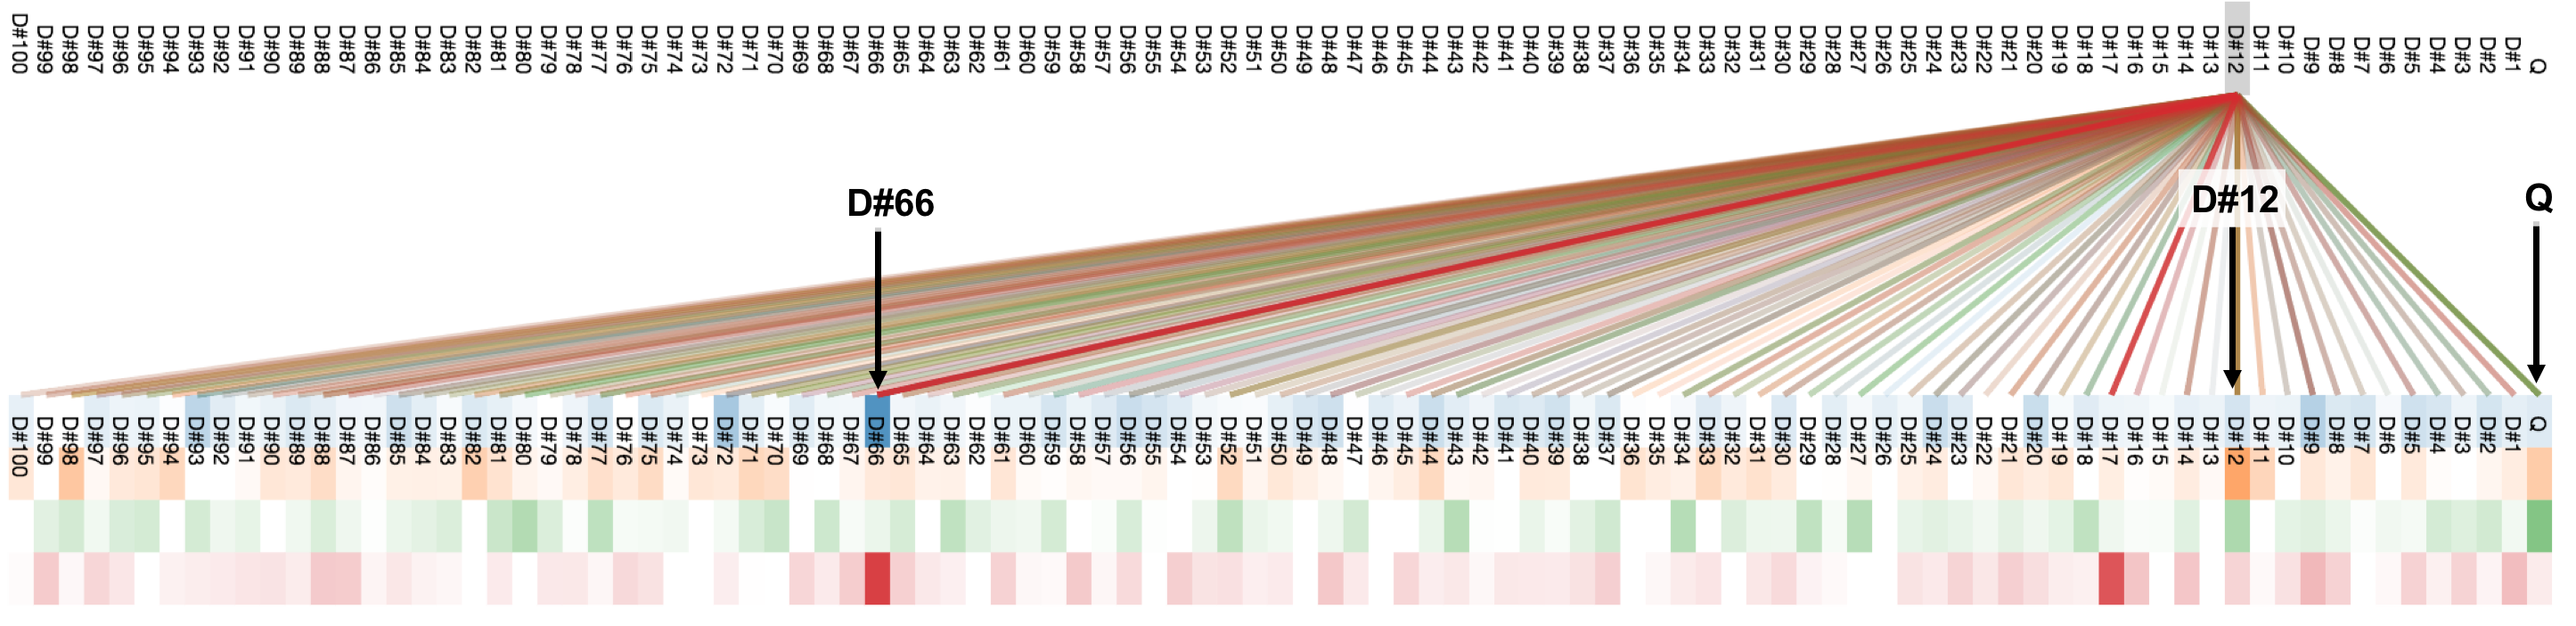
\includegraphics[width=\textwidth]{04-part-03/chapter-06/figs_and_tables/fig_att_tracrnet_step3.png}
        \caption{\label{fig:attention_vis_a}Attention distribution %over different documents and the question 
        when transforming the document at rank 12, in step\#3 of multihop reasoning.}
    \end{subfigure}%
    \vfill
    \begin{subfigure}[t]{\textwidth}
        \centering
        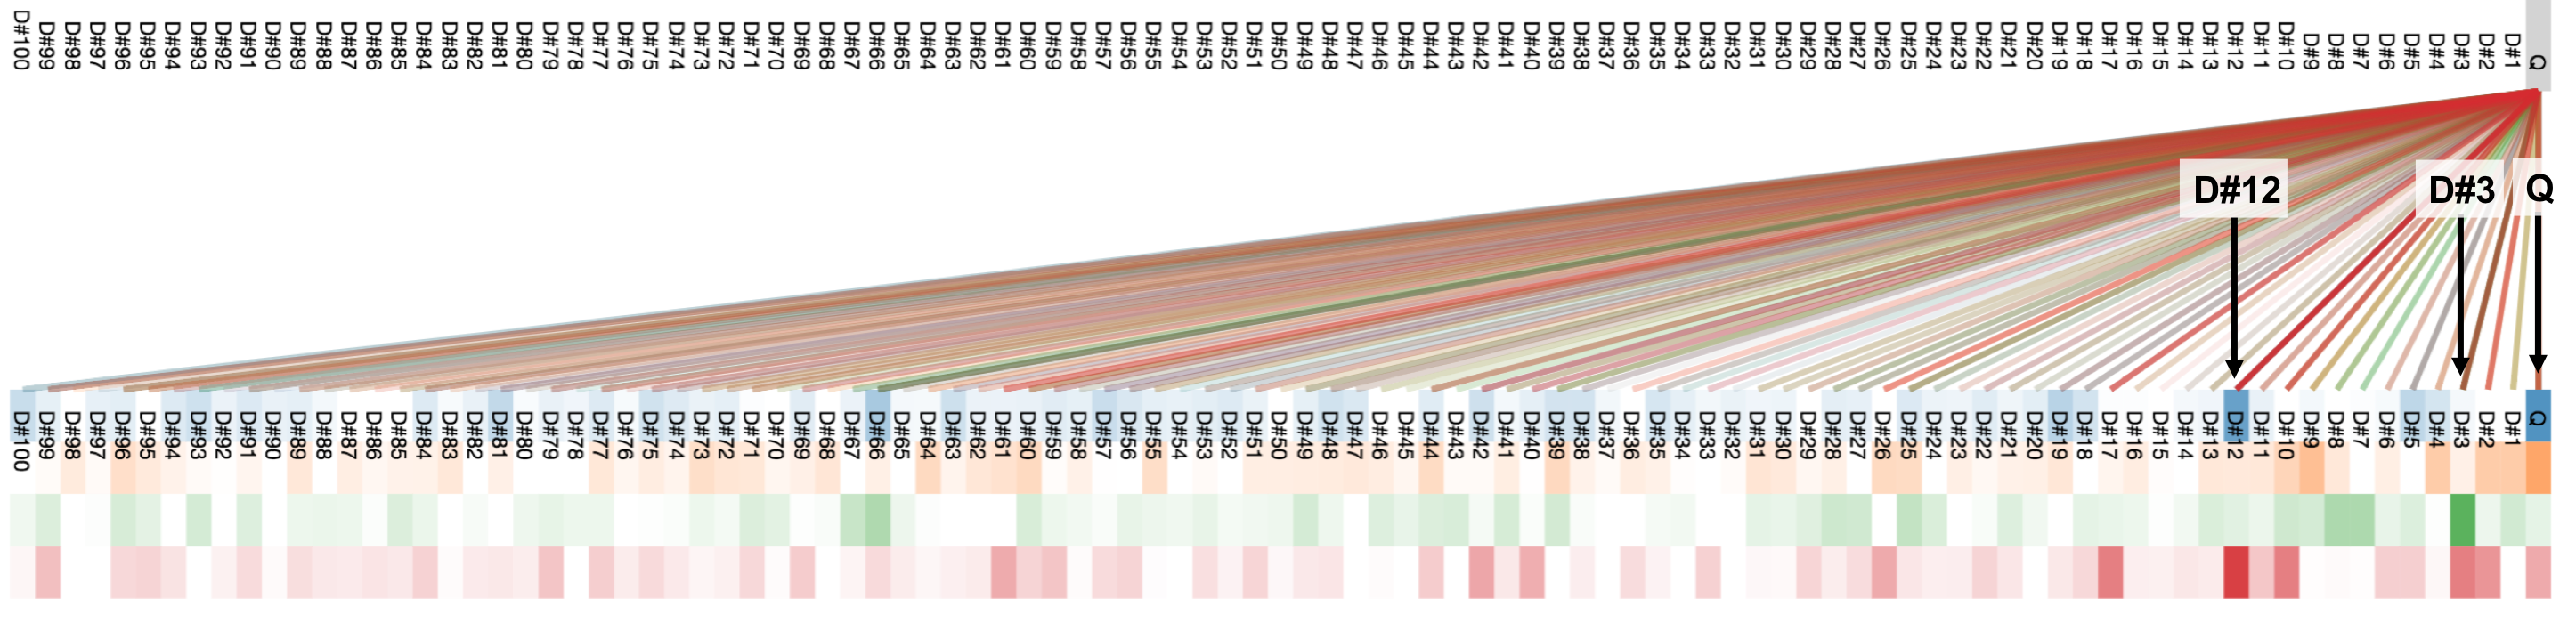
\includegraphics[width=\textwidth]{04-part-03/chapter-06/figs_and_tables/fig_att_tracrnet_step7.png}
        \caption{\label{fig:attention_vis_b}Attention distribution %over different documents and the question 
        when transforming the question, in step\#7 of multihop reasoning.}
    \end{subfigure}
     \caption{Visualization  of multi-head self-attention on Multihop Reasoning layer of \tracrnet. 
     (Best viewed in color.)}
     \label{fig:attention_vis}
\end{figure}

On all measures and datasets, the performance drops when we remove the \emph{Multihop Reasoning} layer. 
The drop in the performance is larger on the Quasar-T dataset than on the SearchQA dataset.
We noticed that trivia questions in Quasar-T, in many cases, contain clauses that should be considered together with and/or operations to be able to give the correct answer. 
For instance, to answer the question ``What Australian food was discovered by John McAdam,'' we should consider that ``the food is Australian'' \emph{and} ``the food is discovered by John McAdam.'' 
In this situation, the chance of having multiple documents each containing one of these facts increases. 
Thus, having multiple supporting documents and the need for reasoning (similar to Example~\ref{fig:example}) will be the exact point where the advantage of the \emph{Multihop Reasoning} layer kicks in.

Another observation here is that when we remove the \emph{Multihop Reasoning} layer, passing word-level embeddings from the encoder to the decoder leads to better EM scores, but not to improved F1 scores. 
The main reason is that, in this situation, access to the input words from the decoder is more explicit. 
This helps the model to get closer to answer extraction than pure answer generation.

For the test example that is presented in Figure~\ref{fig:example}, we observed that all baseline models output ``Georges Braque'' which is extracted from the document at rank~1. 
However, unlike all the baselines, \tracrnet returns the correct answer. 
We looked into the attention distributions in the \emph{Multihop Reasoning} layer of \tracrnet at different steps (of the employed Universal Transformer with 12 depth-wise recurrent steps). 
We were able to find a relation between attention distributions and the reasoning steps that are needed to give the correct answer to this question. 
We illustrate this in Figure~\ref{fig:attention_vis}.

Figure~\ref{fig:attention_vis_a} presents the attention distribution over all documents and the question while encoding the document at rank~12 at step~3. 
\tracrnet has a high level of attention for the document at rank~66 using heads~1 and~4 (blue and red) as well as for the question using head~3 (green) while transforming the document at rank~12. 
This is in accordance with the fact that the model first needs to update the information encoded in the document at rank 12 with the fact that ``Malaga is a city in Spain'' from the document at rank~66. 
Later, at step~7, while encoding the question (Figure~\ref{fig:attention_vis_b}), \tracrnet attends over document 12, which has information about ``Picasso who is a Spanish artist'' (updated in step~3) using heads~1 and~4 and document~3, which contains information about ``Picasso as a co-founder of Cubism'' using head~2 (green). 

\subsubsection{Impact of the number of documents}
As we explained before, unlike most of the previous work that filters candidate documents and narrows down the set of documents under consideration to either a single document or a small set of highly relevant documents before applying an answer extractor to them, \tracrnet uses the full set of candidate documents retrieved by the search engine during the entire process of generating the answer. 
This is of great advantage as our analysis shows that, for some questions, the correct answer can only be extracted when considering information from low-ranked documents that are not immediately relevant to the question.
However, this can potentially come at the cost of (1)~efficiency, as we need to process a larger input, and of (2)~performance, as there will be more noisy and non-relevant documents when we go down the ranked list of candidate documents. 
%
Making use of self-attentive feed-forward neural networks as building blocks of \tracrnet brings the ability of full per-symbol parallelization and leads to an enormous speedup on encoding the input documents. This lets the model encode a larger set of candidate documents efficiently. 

\begin{figure}[!t]
 \centering
 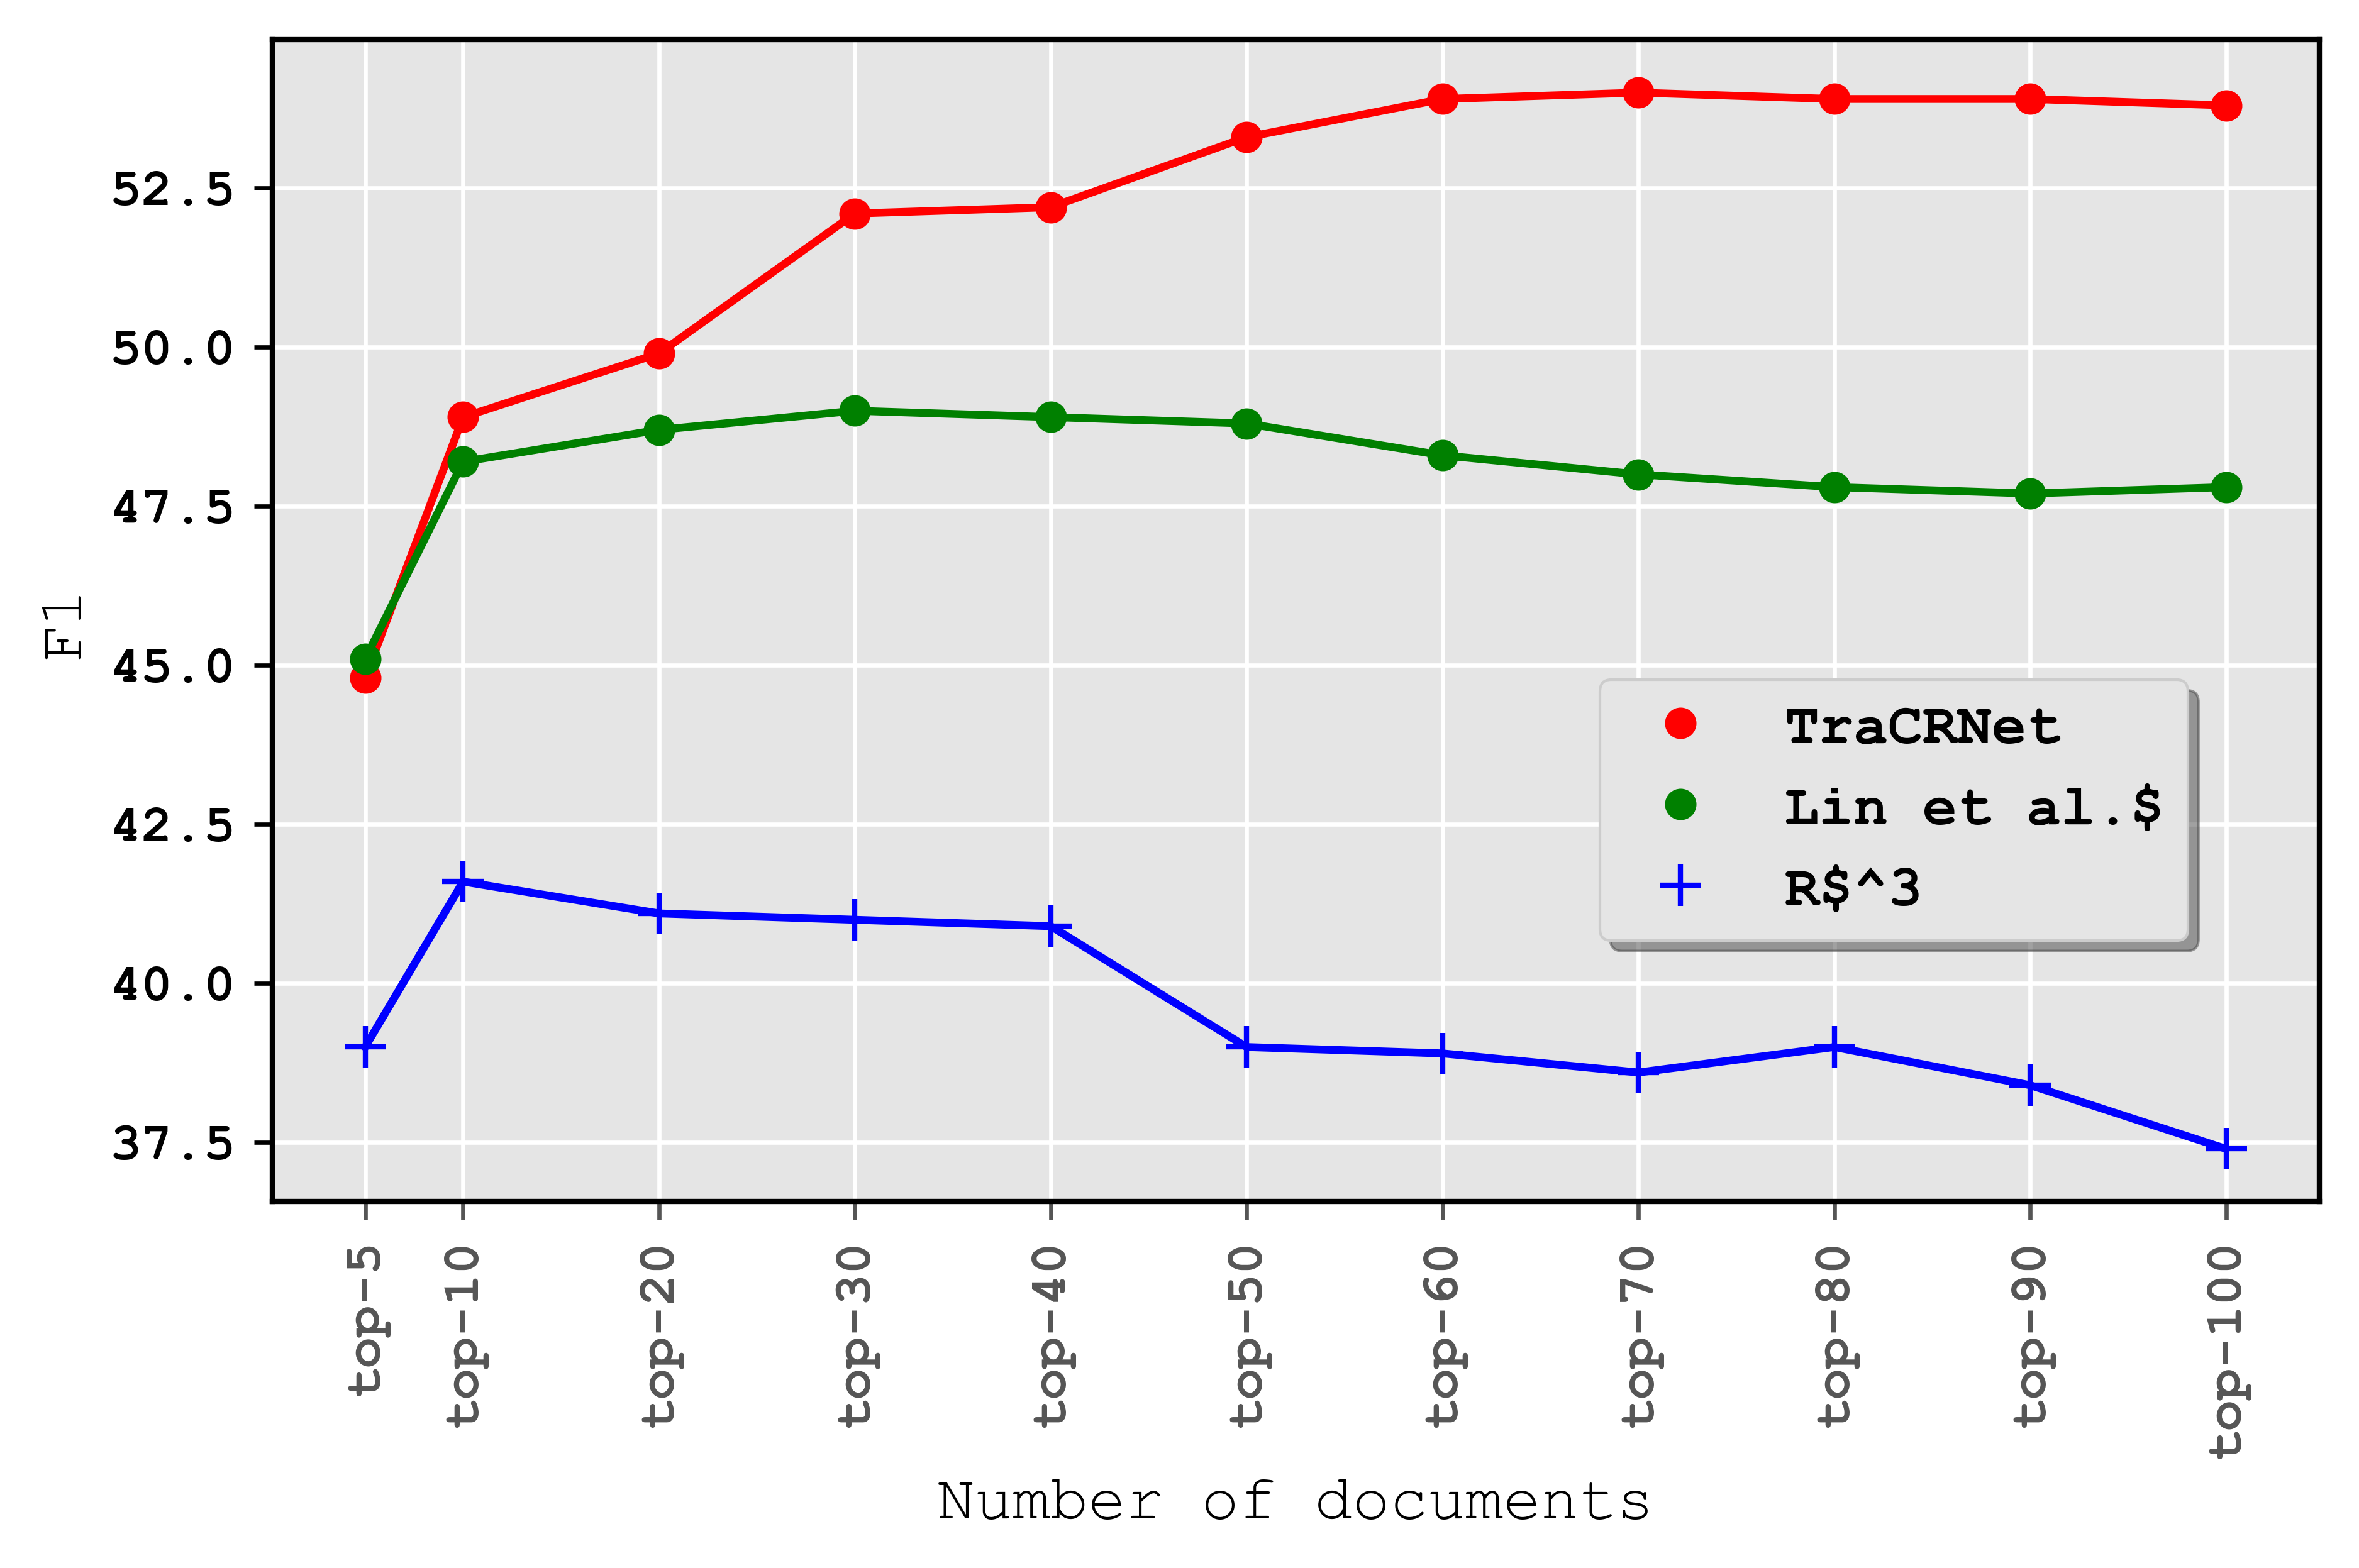
\includegraphics[width=0.6\textwidth]{04-part-03/chapter-06/figs_and_tables/plot_different_num_docs.png}
  %\vspace{5pt}
 \caption{Performance in terms of F1 of \tracrnet and baselines (R$^3$~\citep{wang2017r} and \citet{lin2018denoising}'s model) with different numbers of candidate documents on Quasar-T dataset.}
 \label{fig:diff_num_docs}
\end{figure}

To study how the performance of \tracrnet is affected by the number of candidate documents, we train and evaluate \tracrnet as well as R$^3$~\citep{wang2017r} and \citet{lin2018denoising}'s model on the Quasar-T dataset, using different numbers of candidate documents associated with each question.\footnote{In this experiment, we just change the initial number of candidates, but we train baseline models with their original setups and do not impose any assumption (e.g., fixing the candidate list) on them.}
%
Figure~\ref{fig:diff_num_docs} presents the performance of these models when they are fed with the top-5, top-10, \ldots, top-100 retrieved documents. 
%
As can be seen, although \citet{lin2018denoising}'s model is pretty good at staying robust when noise increases (it is designed to learn from distant supervision), increasing the number of candidate documents eventually leads to a small drop in performance of both baselines due to the noise in the low-ranked documents. 
However, \tracrnet not only controls the effect of noisy low-ranked documents by calibrating their effect on inferring the final answer through self-attention, but it also keeps improving as we increase the number of documents as it can exploit any useful information contained in low-ranked documents which can help better understand the question or perform reasoning.





\section{Conclusion}
In this chapter we focused on addressing \textbf{\resqname{c6}}: ``\emph{\resqcontent{c6}}''.
We introduced the Universal Transformer to address \textbf{\resqname{c6.1}}, a generalization of the Transformer model that extends its theoretical capabilities, by introducing the recurrent inductive bias in depth. 
We have employed the Universal Transformer in on a wide range of challenging sequence modeling tasks, such as language understanding but also a variety of algorithmic tasks, to address \textbf{\resqname{c6.2}} and showed that it produces state-of-the-art results by addressing a key shortcoming of the standard Transformer. The Universal Transformer combines the following key properties into one model:

\textbf{Weight sharing}: Following intuitions behind weight sharing found in CNNs and RNNs, we extend the Transformer with a simple form of weight sharing that strikes an effective balance between inductive bias and model expressivity, which we show extensively on both small and large-scale experiments.

\textbf{Conditional computation}: In our goal to build a computationally universal machine, we equipped the Universal Transformer with the ability to halt or continue computation through a recently introduced mechanism, which shows stronger results compared to the fixed-depth Universal Transformer.

By adding computational capacity and recurrence in processing depth, we hope that further improvements beyond the basic Universal Transformer presented here will help us build learning algorithms that are both more powerful, data efficient, and generalize beyond the current state-of-the-art.

In Part~\ref{part3} of the thesis, we focused on addressing \textbf{\resqname{p3}}: ``\emph{\resqcontent{p3}}''.
we explored the idea of injecting inductive biases into learning algorithms to improve their data-efficiency and generalization. This in fact is defining an innate prior knowledge for the learning algorithms that can eventually help overcoming the challenging problem of poverty of stimulus.

